\UseRawInputEncoding
\documentclass[a4paper,openany,12pt]{book}
\usepackage[spanish, es-ucroman]{babel}
\usepackage[utf8]{inputenc}
\usepackage{fancyhdr}
\usepackage{graphicx}
\usepackage[inner=3.0cm,outer=2.5cm,top=3cm,bottom=3cm]{geometry}%margen 2.54
\usepackage{hlundef}
\usepackage{tesis}
\usepackage[printonlyused]{acronym}
\usepackage{breakcites}
\usepackage{color,soul}
\usepackage{ae}
\usepackage[usenames,dvipsnames,table,xcdraw]{xcolor}
\usepackage{amsmath}
\usepackage{multirow}
\usepackage[inline]{enumitem}
\usepackage{tikz,pgfplots,pgfplotstable}
\usepackage{capt-of}
\usepackage{csvsimple}
\usepackage[breaklinks]{hyperref}
\setlength{\parindent}{1.27cm}
\usepackage[acronym]{glossaries} % paquete de acrónimos
\usepackage{caption}
%\usepackage{subcaption}
\usepackage{booktabs}
\usepackage{enumitem}
\usepackage[colorinlistoftodos]{todonotes}
\usepackage{mathrsfs}
\newtheorem{proposicion}{Proposición}[section]
\usepackage{amsfonts}
\usepackage{etoolbox}
\usepackage[group-separator={,}]{siunitx}
\usepackage{graphicx} 
\usepackage{adjustbox} % también para rotar
\usepackage{array} % Para definir ancho tabla
\usepackage{booktabs}
\newcommand{\ra}[1]{\renewcommand{\arraystretch}{#1}}
\setcounter{secnumdepth}{3}
\pgfplotsset{compat=1.13}
\usepgfplotslibrary{colormaps}
\usepackage{sidecap}
\sidecaptionvpos{figure}{b}
\sidecaptionvpos{table}{b}
\usepackage{natbib}
\setcitestyle{round}
\usepackage{tikz-qtree}
\usepackage{arydshln}
\usetikzlibrary{shapes.geometric, arrows, decorations.pathreplacing, shadows,trees, positioning, calc, tikzmark, spy, mindmap, matrix}
\tikzstyle{roundedFrame} = [rectangle, text centered, rounded corners, draw=gray]
\tikzstyle{input} = [rectangle,text centered, draw=none]
\tikzstyle{emptyFrame} = [rectangle,text centered, draw=white]
\tikzstyle{frame} = [rectangle, text centered, draw=gray]
\tikzstyle{arrow} = [thick,->,>=stealth]
\usepackage{pifont} % DING
% Encabezados de capítulo y sección (APA7: Nivel 1 centrado en negrita,
% Nivel 2 alineado a la izquierda en negrita y del mismo tamaño que el cuerpo)
\usepackage[T1]{fontenc}
\usepackage{titlesec, blindtext, color}
\definecolor{gray75}{gray}{0.75}
\titleformat{\chapter}[block]{\Huge\bfseries}{\thechapter.}{0.8em}{}
\titleformat{\section}{\normalfont\bfseries}{\thesection}{0.8em}{}
% Nuevos comandos para diagrama de gantt
% A package which allows simple repetition counts and some useful commands
\usepackage{forloop}
\newcounter{loopcntr}
\newcommand{\rpt}[2][1]{%
  \forloop{loopcntr}{0}{\value{loopcntr}<#1}{#2}%
}
\newcommand{\on}[1][1]{
  \forloop{loopcntr}{0}{\value{loopcntr}<#1}{&\cellcolor{gray75}}
}
\newcommand{\off}[1][1]{
  \forloop{loopcntr}{0}{\value{loopcntr}<#1}{&}
}
\usepackage[nottoc,notlof,notlot,notbib]{tocbibind}
\usepackage{listings}
\setlength{\headheight}{15pt}

% Para definir ancho tabla
\newcolumntype{L}{>{\centering\arraybackslash}m{4cm}}
\usepackage[caption=false]{subfig}
\usepackage{dsfont}
\usepackage[ruled,vlined]{algorithm2e}

\newtheorem{defn}{Definition}[section]
\pagenumbering{Roman}

\title{SISTEMA DE GESTIÓN DE RUTAS ÓPTIMAS EN CUSCO:\\ ANÁLISIS COMPARATIVO DE ALGORITMOS GREEDY, DIVIDE Y VENCERÁS, PROGRAMACIÓN DINÁMICA Y BACKTRACKING}
\autor1{Amilcar Estacio Medrano}
\codigoautor1{200822}
\autor2{Kevin Heli Choquecahua Gutierrez}
\codigoautor2{245570}
\autor3{Jeliel Enrique Aramburu}
\codigoautor3{210927}
\asesor{Mg. Karla Catherine Rojas Pedraza}
\coasesor{}

\addto\captionsspanish{%
    \renewcommand{\bibname}{Referencias}
    \renewcommand{\listtablename}{Índice de Tablas}
    \renewcommand{\listfigurename}{Índice de Figuras}
}

\begin{document}
%%%%%%%%%%%%%%%%%%%%%%%%%%%%%%%%%%%%%%%%%%%%%%%%%%%%%%%%%%%%%%%%%%%%
% a) Portada
\maketitle

%%%%%%%%%%%%%%%%%%%%%%%%%%%%%%%%%%%%%%%%%%%%%%%%%%%%%%%%%%%%%%%%%%%%
% Lista de Acrónimos
\chapter*{Lista de Acrónimos}
\addcontentsline{toc}{chapter}{Lista de Acrónimos}

\begin{description}[leftmargin=3cm, style=nextline]
    \item[APA] American Psychological Association
    \item[B\&B] Branch and Bound (Ramificación y Poda)
    \item[CVRP] Capacitated Vehicle Routing Problem (Problema de Enrutamiento de Vehículos con Capacidad)
    \item[DFS] Depth-First Search (Búsqueda en Profundidad)
    \item[DyV] Divide y Vencerás (Divide and Conquer)
    \item[EPIIS] Escuela Profesional de Ingeniería Informática y de Sistemas
    \item[GPS] Global Positioning System (Sistema de Posicionamiento Global)
    \item[GUI] Graphical User Interface (Interfaz Gráfica de Usuario)
    \item[JSON] JavaScript Object Notation (Notación de Objetos de JavaScript)
    \item[OSM] OpenStreetMap
    \item[PD] Programación Dinámica (Dynamic Programming)
    \item[TSP] Travelling Salesperson Problem (Problema del Viajante de Comercio)
    \item[UNSAAC] Universidad Nacional de San Antonio Abad del Cusco
    \item[VRP] Vehicle Routing Problem (Problema de Enrutamiento de Vehículos)
    \item[WGS84] World Geodetic System 1984 (Sistema Geodésico Mundial 1984)
\end{description}


%%%%%%%%%%%%%%%%%%%%%%%%%%%%%%%%%%%%%%%%%%%%%%%%%%%%%%%%%%%%%%%%%%%%
% Agradecimientos
\chapter*{Agradecimientos}
\addcontentsline{toc}{chapter}{Agradecimientos}

Agradecemos a la Universidad Nacional de San Antonio Abad del Cusco (UNSAAC) y a la Escuela Profesional de Ingeniería Informática y de Sistemas por brindarnos la formación académica y científica necesaria para el desarrollo de este proyecto.

Expresamos nuestra sincera gratitud a la docente del curso de Programación III, Mg. Karla Catherine Rojas Pedraza, por sus valiosas orientaciones pedagógicas, exigencia metodológica y retroalimentación constante durante el semestre académico. Asimismo, extendemos nuestro reconocimiento a nuestros compañeros de equipo por el compromiso y esfuerzo compartido a lo largo de cada fase de este trabajo.


%%%%%%%%%%%%%%%%%%%%%%%% list of content %%%%%%%%%%%%%%%%%%%%%%%%
% c) Índice general, tablas y figuras
\tableofcontents
\listoftables
\addcontentsline{toc}{chapter}{Índice de Tablas}
\listoffigures
\addcontentsline{toc}{chapter}{Índice de Figuras}

%%%%%%%%%%%%%%%%%%%%%%%%%%%%%%%%%%%%%%%%%%%%%%%%%%%%%%%%%%%%%%%%%%%%
% d) Resumen y Abstract
\chapter*{Resumen}
\addcontentsline{toc}{chapter}{Resumen}

El presente trabajo desarrolla un sistema de gestión de rutas óptimas para reparto de pedidos en la ciudad del Cusco, implementado como aplicación de escritorio en Python con interfaz gráfica basada en Tkinter. El problema central consiste en determinar, de forma eficiente, qué pedidos debe atender un repartidor y en qué orden visitarlos, minimizando la distancia total recorrida y respetando restricciones de capacidad del vehículo y calles cerradas en la red vial. Para resolverlo se implementaron, desde cero y sin librerías de optimización externas, cuatro paradigmas algorítmicos: (1) un algoritmo \textit{Greedy} de vecino más cercano para construcción de ruta; (2) \textit{Merge Sort} (Divide y Vencerás) para ordenamiento de pedidos; (3) \textit{Knapsack 0/1} y \textit{Held-Karp} (Programación Dinámica) para selección óptima de pedidos y ruta TSP exacta; y (4) \textit{Backtracking} con poda de ciclos para exploración de rutas alternativas con calles bloqueadas. Los \textit{benchmarks} empíricos confirmaron la complejidad teórica: Held-Karp alcanzó 42.2 ms para $n=12$ pedidos con un speedup del Greedy de $138.8\times$, mientras que el gap de suboptimalidad del Greedy creció de 0\% en $n=3$ a 14.81\% en $n=12$. El Backtracking encontró entre 3 y 9 rutas alternativas en menos de 1.1 ms en cuatro escenarios del grafo de Cusco. El sistema resultante es estable, visualmente verificable y permite reproducir todos los escenarios de prueba de forma interactiva.

\textit{Palabras clave:} rutas óptimas, algoritmos greedy, programación dinámica, backtracking, Held-Karp, Cusco, TSP, Knapsack

\chapter*{Abstract}
\addcontentsline{toc}{chapter}{Abstract}

This work presents an optimal route management system for parcel delivery in the city of Cusco, implemented as a Python desktop application with a Tkinter graphical interface. The road network is modelled as a directed graph of 20 points of interest and 64 connections weighted by real street lengths from OpenStreetMap; shortest distances between places are precomputed with a hand-written Dijkstra algorithm. On top of this model, the four required paradigms were implemented without external optimization libraries: (1) \textit{Greedy}, with the nearest-neighbour heuristic and the assignment of urgent orders to the closest courier; (2) \textit{Divide and Conquer}, which splits the city at the median alternating latitude and longitude, both into zones of $K$ orders and into one zone per courier; (3) \textit{Dynamic Programming}, with the 0/1 Knapsack to load the vehicle and Held-Karp for the exact tour; and (4) \textit{Backtracking}, which enumerates every simple path between two places while avoiding closed streets, with optional bound-based pruning. Measurements confirmed the Big-O analysis: Held-Karp took 22.2 ms for $n=12$ points against 0.017 ms for Greedy, while the greedy tour was up to 24.5\% longer than the optimum. In the case stated by the assignment, from San Blas to Wanchaq, Backtracking found all 27 simple paths and the shortest one (1,778.6 m); pruning kept that same path while visiting 20 states instead of 146. Splitting the 30 orders into three zones, one per courier, reduced the total distance from 43.4 km (a single greedy courier) to 30.2 km. The system passes 39 unit tests and an automated interface test that exercises every feature.

\textit{Keywords:} optimal routes, greedy algorithms, divide and conquer, dynamic programming, backtracking, Held-Karp, 0/1 knapsack, Dijkstra, Cusco


\setlength{\tabcolsep}{6pt}
\renewcommand{\arraystretch}{1}
\clearpage
\pagenumbering{arabic}
%%%%%%%%%%%%%%%%%%%%%%%%%%%%%%%%%%%%%%%%%%%%%%%%%%%%%%%%%%%%%%%%%%%%%
% Contenido del informe técnico
%%%%%%%%%%%%%%%%%%%%%%%%%%%%%%%%%%%%%%%%%%%%%%%%%%%%%%%%%%%%%%%%%%%%%
\chapter{Introducción}

El problema de la distribución eficiente de bienes en entornos urbanos es uno de los desafíos logísticos más relevantes tanto en la industria como en el campo del diseño algorítmico. En ciudades como el Cusco, cuya red vial histórica presenta calles angostas, sentidos únicos, zonas peatonales y calles frecuentemente bloqueadas por actividades culturales o de mantenimiento, la planificación manual de rutas de reparto resulta especialmente compleja e ineficiente.

El presente proyecto, desarrollado en el marco del curso de Programación III de la Escuela Profesional de Ingeniería Informática y de Sistemas (EPIIS) de la Universidad Nacional de San Antonio Abad del Cusco (UNSAAC), aborda esta problemática mediante la construcción de un sistema de gestión de rutas óptimas implementado como aplicación de escritorio en Python. El sistema integra una interfaz gráfica de usuario (GUI) basada en Tkinter que permite visualizar la red vial de Cusco ---20 lugares de interés unidos por calles reales de OpenStreetMap---, cerrar calles, gestionar pedidos de reparto y ejecutar cuatro paradigmas algorítmicos fundamentales del diseño de algoritmos: \textit{Greedy}, \textit{Divide y Vencerás}, \textit{Programación Dinámica} y \textit{Backtracking}.

El trabajo no se limita a la implementación funcional de los algoritmos, sino que incluye un análisis riguroso de su complejidad computacional temporal y espacial en notación Big-O, así como la ejecución de \textit{benchmarks} empíricos que permiten comparar el rendimiento real de cada paradigma ante diferentes volúmenes de datos. De este modo, el sistema sirve simultáneamente como herramienta práctica de apoyo a la logística urbana y como plataforma de demostración pedagógica de los paradigmas algorítmicos estudiados durante el semestre.

El documento se organiza de la siguiente manera: el Capítulo 2 describe el planteamiento del problema y su justificación; el Capítulo 3 establece los objetivos del proyecto; el Capítulo 4 desarrolla el marco teórico de los algoritmos implementados; el Capítulo 5 formula la hipótesis de trabajo; el Capítulo 6 describe la metodología de desarrollo; el Capítulo 7 presenta los resultados obtenidos y su discusión comparativa; y el Capítulo 8 expone las conclusiones y recomendaciones finales.

\chapter{Planteamiento del Problema}

\section{Descripción de la Situación Problemática}

La ciudad del Cusco posee una red vial de carácter histórico que impone restricciones singulares a la movilidad urbana. Calles con ancho insuficiente para vehículos de carga, zonas de tráfico restringido en el Centro Histórico, sentidos únicos de circulación, y cierres temporales frecuentes por eventos culturales o trabajos de mantenimiento, hacen que la planificación manual de rutas de distribución sea altamente ineficiente. A esto se suma la creciente demanda de servicios de reparto a domicilio, que ha crecido de manera sostenida en los últimos años tanto en el ámbito nacional como en la región del Cusco.

Las empresas y emprendimientos locales que realizan reparto de pedidos —restaurantes, farmacias, tiendas de abarrotes, comercio electrónico local— carecen, en su mayoría, de herramientas computacionales que les permitan determinar de forma sistemática qué pedidos priorizar cuando la capacidad del vehículo es limitada, y en qué orden visitarlos para minimizar el tiempo y la distancia recorrida. En la práctica, esta decisión se delega al criterio empírico del repartidor, lo que conduce a rutas subóptimas, mayor consumo de combustible, entregas tardías y reducción de la capacidad de atención diaria.

Desde el punto de vista algorítmico, el problema de la selección óptima de pedidos bajo restricción de capacidad corresponde al problema de la Mochila 0/1 (\textit{Knapsack 0/1}), mientras que la determinación del orden de visita óptimo es una instancia del Problema del Viajante de Comercio (\textit{Travelling Salesperson Problem}, TSP). Ambos pertenecen a la clase de problemas NP-difíciles para los cuales la Programación Dinámica ofrece soluciones exactas de complejidad exponencial, y las heurísticas \textit{Greedy} constituyen alternativas prácticas de complejidad polinomial. La incorporación de restricciones de calles bloqueadas introduce la necesidad de técnicas de búsqueda exhaustiva como el \textit{Backtracking}, mientras que la organización y preprocesamiento de los pedidos se beneficia del paradigma \textit{Divide y Vencerás}.

Este proyecto responde a la necesidad académica de contrastar empíricamente estos cuatro paradigmas sobre un caso de uso concreto y relevante localmente, analizando sus diferencias de rendimiento y calidad de solución.

\section{Problema General}

¿En qué medida el diseño e implementación de un sistema computacional que aplica los paradigmas algorítmicos Greedy, Divide y Vencerás, Programación Dinámica y Backtracking permite gestionar eficientemente las rutas de reparto en la ciudad del Cusco, optimizando la distancia total recorrida y el cumplimiento de restricciones operativas?

\section{Problemas Específicos}

El estudio toma en cuenta los siguientes problemas específicos:
\begin{itemize}
    \item ¿Cómo afecta la elección del paradigma algorítmico (Greedy vs. Programación Dinámica) a la calidad de la selección de pedidos bajo restricción de capacidad, medida como distancia total de la ruta generada?
    \item ¿Cuál es la complejidad temporal y espacial real, medida empíricamente, de cada uno de los cuatro algoritmos implementados en función del número de pedidos activos?
    \item ¿En qué condiciones del grafo vial (número de aristas bloqueadas, densidad de la red) el algoritmo de Backtracking logra encontrar rutas alternativas viables en tiempo aceptable para un usuario interactivo?
\end{itemize}

\section{Justificación}

La justificación de este trabajo es de naturaleza académica y práctica. En el plano académico, el proyecto constituye una demostración integral de cuatro de los paradigmas algorítmicos más importantes del diseño de algoritmos, aplicados sobre un problema de optimización combinatoria real. La implementación desde cero de cada algoritmo —sin recurrir a librerías de optimización externas— permite a los integrantes del equipo comprender en profundidad la estructura y el comportamiento computacional de cada paradigma, lo que resulta esencial para la formación en Ingeniería Informática y de Sistemas.

En el plano práctico, el sistema desarrollado demuestra que es posible construir, con recursos computacionales modestos y en Python, una herramienta de apoyo a la decisión logística para pequeñas y medianas empresas de reparto en Cusco. Si bien el grafo vial utilizado es una simulación con 20 nodos de referencia geográfica real, la arquitectura modular del sistema permite su extensión futura con datos reales obtenidos de OpenStreetMap.

La comparación cuantitativa entre algoritmos, respaldada por \textit{benchmarks} empíricos y análisis Big-O, añade valor pedagógico al permitir visualizar de forma directa la diferencia entre complejidad polinomial y exponencial en un contexto aplicado.

\chapter{Objetivos de la Investigación}
\label{ch:objetivos_ph}

\section{Objetivo General}

Diseñar e implementar un sistema de escritorio en Python que gestione pedidos de reparto y genere rutas óptimas en un grafo vial simulado de la ciudad del Cusco, integrando y comparando cuatro paradigmas algorítmicos —Greedy, Divide y Vencerás, Programación Dinámica y Backtracking— mediante análisis de complejidad Big-O y benchmarks empíricos, con el fin de determinar el paradigma más adecuado según el tamaño del problema y las restricciones operativas.

\section{Objetivos Específicos}

\begin{itemize}
    \item Implementar desde cero los algoritmos Greedy de selección por densidad, Merge Sort (Divide y Vencerás), Knapsack 0/1 y Held-Karp (Programación Dinámica), y Backtracking con poda de calles bloqueadas, verificando su correctitud mediante pruebas unitarias con \texttt{pytest}.
    \item Derivar y documentar la complejidad temporal y espacial Big-O de cada algoritmo implementado, comparando el crecimiento teórico con los tiempos de ejecución medidos experimentalmente para entre 3 y 15 pedidos activos.
    \item Desarrollar una interfaz gráfica de usuario (GUI) con Tkinter que permita visualizar el grafo vial, gestionar pedidos y repartidores, ejecutar cada algoritmo de forma interactiva, y presentar los resultados de comparación en gráficos de rendimiento.
\end{itemize}

\chapter{Marco Teórico}

En este capítulo se presentan los fundamentos teóricos que sustentan el diseño e implementación del sistema: el modelo de la red vial, los paradigmas algorítmicos aplicados, el análisis de complejidad de cada algoritmo implementado y la notación empleada.

\section{Antecedentes}

\citet{dantzig1959truck} formularon el Problema de Enrutamiento de Vehículos (VRP) como generalización del TSP con múltiples vehículos y capacidad limitada, estableciendo las bases formales del problema que este proyecto aborda en escala reducida. La planificación óptima de rutas es NP-difícil en el caso general, lo que motiva el uso combinado de heurísticas y algoritmos exactos de costo exponencial acotado.

\citet{dijkstra1959note} propuso el algoritmo de caminos mínimos desde un origen en grafos con pesos no negativos, que en este proyecto se usa para calcular la distancia por calles entre cada par de lugares de interés.

\citet{held1962dynamic} propusieron el algoritmo de Programación Dinámica para el TSP que lleva su nombre, reduciendo la complejidad de la fuerza bruta $O(n!)$ a $O(n^2 2^n)$ mediante memoización sobre subconjuntos de nodos visitados.

\citet{rosenkrantz1977analysis} analizaron heurísticas constructivas para el TSP, entre ellas la del vecino más cercano, base del enfoque Greedy implementado, y demostraron que, en instancias métricas, puede alejarse del óptimo en un factor que crece con $\log n$; en una red dirigida como la de este proyecto ni siquiera esa cota está garantizada.

\citet{cormen2022introduction} proporcionan el tratamiento formal de los paradigmas implementados y del Teorema Maestro empleado en el análisis de recurrencias. \citet{toth2014vehicle} contextualizan la selección y secuenciación de pedidos con capacidad (CVRP) dentro de la logística moderna.

\section{Bases Teóricas}

\subsection{Modelo de la red vial}

La ciudad se representa con un grafo dirigido y ponderado $G=(V,E)$. Cada vértice $v\in V$ es uno de los 20 lugares de interés (Plaza de Armas, San Blas, Wanchaq, etc.), con latitud, longitud y sector. Cada arco $(u,v)\in E$ es un recorrido por calles reales entre dos lugares, obtenido de OpenStreetMap con perfil vehicular: su peso $w(u,v)$ es la suma de las longitudes de los tramos de calle, en metros, y conserva la polilínea para dibujarlo. Como existen calles de un solo sentido, $w(u,v)$ puede ser distinto de $w(v,u)$, o uno de los dos arcos puede no existir; la red usada tiene $|E|=64$ arcos dirigidos: 20 pares en ambos sentidos y 24 arcos de un solo sentido.

El grafo se almacena como diccionario de adyacencia \texttt{adyacencia[u][v]} $\to$ arista, que ocupa $O(|V|+|E|)$, recorre los vecinos de un nodo en $O(\deg(u))$ y consulta una arista concreta en $O(1)$ promedio. Se eligió frente a la matriz de adyacencia porque la red urbana es dispersa (en promedio 3.2 arcos de salida por lugar), de modo que la matriz desperdiciaría $O(|V|^2)$ espacio y obligaría a recorrer filas completas para obtener vecinos. Cada arista lleva además un indicador \texttt{activa}: cerrar una calle lo pone en falso en ambos sentidos sin modificar la estructura del grafo.

\textbf{Distancias mínimas (Dijkstra).} Los algoritmos de ruta necesitan la distancia por calles entre lugares que no son vecinos directos. Se ejecuta Dijkstra con cola de prioridad (\texttt{heapq}) desde cada uno de los $|V|$ lugares, ignorando las calles cerradas:
\begin{equation}
    T_{\text{matriz}} = |V|\cdot O\big((|V|+|E|)\log|V|\big), \qquad S_{\text{matriz}} = O(|V|^2).
\end{equation}
El resultado se guarda en caché y se invalida automáticamente cada vez que se cierra o reabre una calle. Con la matriz disponible, la distancia entre dos lugares se consulta en $O(1)$, y por eso los algoritmos siguientes suponen $d(u,v)$ de costo constante.

La distancia en línea recta (fórmula de Haversine) se usa solo para asignar un pedido nuevo, ingresado por coordenadas, al lugar de interés más cercano, y para mostrar en la interfaz el factor de desvío entre la línea recta y el recorrido por calles.

\subsection{Estructuras, ordenación y búsqueda}

\begin{itemize}
    \item \textbf{Merge Sort}: divide la lista en dos mitades, las ordena recursivamente y las mezcla. $T(n)=2T(n/2)+\Theta(n)=\Theta(n\log n)$ en todos los casos; espacio $O(n)$; es estable.
    \item \textbf{Quick Sort} (partición de Lomuto, pivote por mediana de tres): $\Theta(n\log n)$ en promedio y $O(n^2)$ en el peor caso; espacio $O(\log n)$ promedio por la pila de recursión.
    \item \textbf{Búsqueda por ID con tabla hash} (\texttt{dict}): construcción $O(n)$, consulta $O(1)$ promedio.
    \item \textbf{Búsqueda binaria} sobre la lista ordenada por ID: $O(\log n)$ comparaciones, espacio $O(1)$.
    \item \textbf{Índice invertido por sector}: \texttt{sector} $\to$ lista de pedidos; construcción $O(n)$ y consulta $O(1)$ por sector.
\end{itemize}

\subsection{Paradigma Greedy}

Un algoritmo \textit{Greedy} construye la solución paso a paso tomando en cada etapa la mejor decisión local, sin reconsiderar decisiones anteriores \citep{cormen2022introduction}. Se aplica en tres puntos:

\textbf{Vecino más cercano.} Desde la posición actual, el repartidor visita el pedido pendiente con menor $d(\text{actual},p)$. En la iteración $i$ se comparan $n-i$ candidatos:
\begin{equation}
    T(n)=\sum_{i=0}^{n-1}(n-i)=\frac{n(n+1)}{2}=O(n^2), \qquad S(n)=O(n).
\end{equation}

\textbf{Pedido de emergencia.} Se asigna el pedido urgente al repartidor con capacidad suficiente cuya distancia por calles al destino sea mínima: una comparación por repartidor, $O(R)$ tiempo y $O(1)$ espacio.

\textbf{Mochila voraz} (solo como referencia de comparación). Ordena los pedidos por valor/kg con Merge Sort y los toma mientras quepan: $O(n\log n)$. No garantiza el óptimo de la mochila 0/1: con pesos $(1,2,3)$, valores $(15,10,30)$ y $W=4$ toma los dos primeros (valor 25), cuando el óptimo es el primero y el tercero (valor 45).

\subsection{Paradigma Divide y Vencerás}

Divide y Vencerás divide el problema en subproblemas del mismo tipo, los resuelve recursivamente y combina sus soluciones \citep{cormen2022introduction}. Se usa para segmentar la ciudad.

\textbf{Partición en zonas de a lo sumo $K$ pedidos.} Si hay más de $K$ pedidos, se ordenan con Quick Sort por latitud (niveles pares) o longitud (niveles impares), se cortan por la mediana y se procesa cada mitad. Como el trabajo no recursivo es ordenar,
\begin{equation}
    T(n)=2T(n/2)+\Theta(n\log n).
\end{equation}
Con $a=b=2$, $n^{\log_b a}=n$ y $f(n)=\Theta(n\log n)=\Theta(n^{\log_b a}\log^1 n)$; por la forma extendida del caso 2 del Teorema Maestro, $T(n)=\Theta(n\log^{2} n)$. (Si la mediana se obtuviera por selección lineal en lugar de ordenar, $f(n)=\Theta(n)$ y el resultado sería $\Theta(n\log n)$.) Después, un repartidor entra a la zona cuyo pedido más cercano esté a menor distancia y la recorre con vecino más cercano. Con $M=n/K$ zonas, esa elección cuesta $\sum_i (M-i)\,K=O(M^2K)=O(n^2/K)$ y las rutas locales $M\cdot O(K^2)=O(nK)$, por lo que el total es $O(n^2/K)$ en tiempo y $O(n)$ en espacio.

\textbf{Una zona por repartidor} (caso de uso del enunciado). Con $R$ repartidores, la ciudad se divide en exactamente $R$ zonas: si $r=1$ la zona es todo el conjunto; si no, se ordena por el eje del nivel, se corta en la proporción $\lfloor r/2\rfloor:\lceil r/2\rceil$ y se resuelve cada parte con ese número de zonas. El árbol tiene profundidad $\lceil\log_2 R\rceil$ y en cada nivel se ordenan $n$ elementos:
\begin{equation}
    T(n,R)=\Theta(n\log n\cdot\log R).
\end{equation}
Cada zona se asigna al repartidor más cercano mediante un emparejamiento voraz sobre los $R^2$ pares ordenados por distancia, $O(R^2\log R + Rn)$, y cada repartidor calcula la ruta \emph{óptima} de su zona con Held-Karp cuando tiene a lo sumo 10 pedidos.

\subsection{Programación Dinámica}

La Programación Dinámica resuelve un problema a partir de subproblemas superpuestos cuyas soluciones se almacenan para no recalcularlas, apoyándose en el principio de optimalidad \citep{bellman1957dynamic}.

\textbf{Mochila 0/1.} Dados $N$ pedidos con peso $w_i$ y valor $v_i$, y una capacidad $W$, se maximiza $\sum v_i$ sujeto a $\sum w_i\le W$. La tabla $dp[i][c]$ guarda el mejor valor usando los primeros $i$ pedidos con capacidad $c$:
\begin{equation}
    dp[i][c]=\begin{cases}dp[i-1][c] & \text{si } w_i>c\\ \max\big(dp[i-1][c],\; v_i+dp[i-1][c-w_i]\big) & \text{si } w_i\le c\end{cases}
\end{equation}
con $dp[0][c]=0$. La solución se reconstruye recorriendo la tabla hacia atrás: el pedido $i$ se eligió si $dp[i][c]\neq dp[i-1][c]$. Como la tabla se indexa con enteros, los pesos se expresan en unidades de 0.1 kg (escala 10), \emph{redondeando los pesos hacia arriba y la capacidad hacia abajo}, lo que garantiza que la carga elegida nunca supere la capacidad real. La complejidad es $O(N\cdot W)$ en tiempo y espacio, con $W$ la capacidad en décimas de kg: es pseudo-polinomial, porque depende del valor numérico de $W$; multiplicar la precisión por 10 multiplica las columnas de la tabla y el tiempo por 10.

\textbf{Held-Karp (TSP exacto).} El estado $(\text{mask},u)$ indica el conjunto de puntos ya visitados, codificado en los bits de un entero, y el punto actual $u$. Con memoización se calcula
\begin{equation}
    C(\text{mask},u)=\min_{v\notin\text{mask}}\big[d(u,v)+C(\text{mask}\cup\{v\},v)\big],
\end{equation}
con caso base $C(\text{todos},u)=d(u,0)$ si se vuelve al inicio o $0$ si el recorrido es abierto. Hay $2^n\cdot n$ estados y cada uno evalúa hasta $n$ transiciones: $O(n^2 2^n)$ tiempo y $O(n\,2^n)$ espacio \citep{held1962dynamic}.

\subsection{Backtracking}

El Backtracking construye la solución de forma incremental y retrocede al agotar las opciones de una decisión. Para encontrar las rutas de un origen a un destino se usa una búsqueda en profundidad (DFS) sobre caminos simples:

\begin{algorithm}[H]
\SetAlgoLined
\KwData{nodo actual $u$, camino, visitados, costo acumulado}
\eIf{$u$ = destino}{guardar una copia del camino y su costo\;}{
  \ForEach{vecino $v$ de $u$ por una calle abierta}{
    \If{$v\notin$ visitados}{
      agregar $v$ a camino y visitados \tcp*{avanzar}
      \textsc{Buscar}$(v,\ldots,\text{costo}+w(u,v))$\;
      quitar $v$ de camino y visitados \tcp*{retroceder}
    }
  }
}
\caption{Backtracking para todas las rutas simples}
\label{alg:backtracking}
\end{algorithm}

Las calles cerradas se excluyen al pedir los vecinos activos, y el conjunto de visitados impide los ciclos. Sin poda, el algoritmo enumera \emph{todas} las rutas simples, como pide el enunciado, y al final se ordenan por distancia para elegir la más corta.

\textbf{Poda por cota (Branch \& Bound).} Opcionalmente se abandona una rama en cuanto su costo parcial iguala o supera la mejor ruta completa encontrada. Como los pesos son no negativos, el costo de una rama solo puede crecer al extenderla: una rama podada nunca terminaría en una ruta más corta, por lo que la poda conserva la ruta óptima y solo reduce el trabajo.

\textbf{Complejidad.} En un grafo de grado medio $b$ y caminos de longitud $d$, el árbol de búsqueda tiene $O(b^d)$ nodos; en el peor caso, un grafo completo, hay $O(V!)$ caminos simples y copiar cada uno cuesta $O(V)$, es decir, $O(V\cdot V!)$. La poda no mejora esta cota asintótica, pero reduce mucho los estados visitados en la práctica. El espacio es $O(V)$ para la pila, el camino y los visitados, más $O(R\cdot V)$ para guardar las $R$ rutas encontradas.

\subsection{Notación Big-O}

$T(n)=O(f(n))$ si existen constantes $c>0$ y $n_0\ge0$ tales que $T(n)\le c\,f(n)$ para todo $n\ge n_0$; $\Theta$ indica además una cota inferior del mismo orden \citep{cormen2022introduction}. Las complejidades de este proyecto, de menor a mayor, son: $O(1)$, $O(\log n)$, $O(n)$, $O(n\log n)$, $O(n\log^2 n)$, $O(n^2)$, $O(N\cdot W)$ (pseudo-polinomial), $O(n^2 2^n)$ y $O(V\cdot V!)$.

\chapter{Hipótesis de Investigación}

\section{Hipótesis General}

La implementación de un sistema computacional que integra los paradigmas algorítmicos Greedy, Divide y Vencerás, Programación Dinámica y Backtracking permite gestionar rutas de reparto en la ciudad del Cusco de forma sistemática y eficiente, con la condición de que el número de pedidos activos no supere 12 para que el algoritmo exacto Held-Karp sea ejecutable en tiempo interactivo (menor a 50 ms en hardware de escritorio estándar).

\section{Hipótesis Específicas}

\begin{itemize}
    \item El algoritmo de Programación Dinámica Held-Karp producirá, en todos los casos evaluados, una distancia de ruta menor o igual a la del Greedy, con un gap de suboptimalidad del Greedy que crecerá con $n$, superando el 10\% a partir de $n \geq 8$ pedidos activos.
    \item El tiempo de ejecución medido empíricamente del algoritmo Held-Karp crecerá de forma exponencial con el número de pedidos $n$, mientras que el tiempo del algoritmo Greedy crecerá de forma polinomial, verificando los órdenes teóricos $O(2^n \cdot n^2)$ y $O(n^2)$, respectivamente.
    \item El algoritmo de Backtracking encontrará todas las rutas alternativas simples entre el nodo origen y destino en el grafo vial, aplicando poda de ciclos eficientemente, con un tiempo de ejecución menor a 2 ms para los pares de nodos evaluados en el grafo de 20 nodos de Cusco.
\end{itemize}

\section{Verificación de Hipótesis}

Tras la ejecución de los \textit{benchmarks} y la revisión de resultados (Capítulo 7), las hipótesis fueron verificadas de la siguiente manera:

\begin{itemize}
    \item \textbf{Hipótesis 1 — Confirmada:} Held-Karp produjo en todos los casos la ruta de menor distancia. El gap del Greedy fue 0\% para $n=3$, creció a 12.29\% para $n=8$ y llegó a 14.81\% para $n=12$, superando el umbral del 10\% a partir de $n=8$ exactamente como se predijo.
    \item \textbf{Hipótesis 2 — Confirmada:} El speedup del Greedy sobre Held-Karp pasó de $7.6\times$ en $n=3$ a $138.8\times$ en $n=12$, crecimiento consistente con la divergencia exponencial esperada. Las curvas teóricas de referencia en la Figura \ref{fig:tiempo_vs_n} confirman el ajuste.
    \item \textbf{Hipótesis 3 — Confirmada:} El Backtracking encontró entre 3 y 9 rutas alternativas en los 4 escenarios evaluados, con tiempos de 0.058 a 1.073 ms, todos menores a 2 ms como se predijo.
\end{itemize}

\chapter{Metodología de la Investigación}

En este capítulo se describe el enfoque metodológico y el procedimiento seguido para diseñar, implementar, verificar y evaluar el sistema.

\section{Tipo de Investigación}

El trabajo es una investigación \textbf{aplicada y experimental}. Es aplicada porque resuelve un problema concreto ---la planificación de rutas de reparto en Cusco--- con conocimientos de algoritmia. Es experimental porque se diseñaron \textit{benchmarks} reproducibles para medir el comportamiento de cada algoritmo y contrastarlo con su análisis Big-O.

\section{Proceso Metodológico}

\subsection{Fase 1: Modelo de datos y red vial}

Se definieron las entidades en \texttt{core/modelos.py} con \texttt{dataclasses}: \texttt{Nodo} (id, nombre, latitud, longitud, sector), \texttt{Arista} (origen, destino, longitud en metros, geometría, nombres de calles y estado \texttt{activa}), \texttt{Pedido} (id, cliente, lugar de destino, coordenadas, sector, prioridad 1--3, peso, volumen y valor), \texttt{Repartidor} (vehículo, lugar de inicio y capacidades de peso y volumen) y \texttt{Ruta}. La clase \texttt{Grafo} guarda los nodos en un diccionario \texttt{id} $\to$ nodo y la adyacencia como diccionario de diccionarios.

La red vial se construyó fuera de línea con \texttt{tools/construir\_red\_vial.py}: se descargó la red de calles de Cusco de OpenStreetMap con perfil vehicular (\texttt{network\_type="drive"}, respetando sentidos de circulación), se ajustó cada uno de los 20 lugares a la intersección más cercana, y cada lugar se conectó con los 3 lugares más cercanos por calles; se añadieron 4 conexiones más para que todo lugar sea alcanzable desde cualquier otro (grafo fuertemente conexo). El peso de cada conexión es la longitud real del camino por calles. El resultado se guardó en \texttt{data/red\_vial\_cache.json} (descarga del 19 de octubre de 2026; datos © OpenStreetMap contributors, licencia ODbL), de modo que la aplicación no necesita Internet ni librerías de grafos para funcionar. Ocho lugares quedaron a más de 60 m de su coordenada original al ajustarse a la intersección más cercana (el mayor, el acceso a Sacsayhuamán, a 268 m); el Anexo B lista los ajustes.

Los datos de prueba son 30 pedidos (\texttt{data/pedidos.json}) distribuidos en los cuatro sectores, con pesos de 1 a 15 kg y prioridades 1 a 3, y 3 repartidores con bicicleta (15 kg), motocicleta (35 kg) y furgoneta (90 kg) que parten de la Plaza de Armas, Av. El Sol y Marcavalle, respectivamente.

\subsection{Fase 2: Implementación algorítmica}

Los algoritmos se implementaron en \texttt{core/}, sin interfaz gráfica, para poder probarlos de forma aislada:
\begin{itemize}
    \item \texttt{core/grafo.py}: Dijkstra con \texttt{heapq}, matriz de distancias mínimas en caché y reconstrucción de caminos.
    \item \texttt{core/estructuras.py}: Merge Sort, Quick Sort, búsqueda binaria, índice hash por ID e índice invertido por sector.
    \item \texttt{core/greedy.py}: vecino más cercano, asignación de emergencia y mochila voraz (de referencia).
    \item \texttt{core/divide\_venceras.py}: partición espacial en zonas de $K$ pedidos y en $R$ zonas, con asignación de una zona por repartidor.
    \item \texttt{core/prog\_dinamica.py}: Mochila 0/1 con tabla y reconstrucción, y Held-Karp con máscara de bits.
    \item \texttt{core/backtracking.py}: búsqueda exhaustiva de rutas simples con poda opcional por cota.
\end{itemize}
No se usaron librerías de optimización ni de grafos (\texttt{networkx}, \texttt{scipy}) en la aplicación, ni las funciones \texttt{sorted()} o \texttt{list.sort()} de Python para las ordenaciones evaluadas. Cada función documenta en su \textit{docstring} la idea del algoritmo y su complejidad temporal y espacial.

\subsection{Fase 3: Interfaz gráfica}

La GUI usa \texttt{tkinter}/\texttt{ttk} con un \texttt{Notebook} de siete pestañas: Red Vial, Pedidos, Greedy, Divide y Vencerás, Programación Dinámica, Backtracking y Comparación Big-O. El mapa usa \texttt{tkintermapview} con tiles de OpenStreetMap cuando hay conexión; si no la hay, la aplicación lo detecta al iniciar y dibuja la red en un \texttt{Canvas} vectorial propio, en el que también se pueden cerrar calles con un clic. Para cumplir el criterio de estabilidad:
\begin{itemize}
    \item Los cálculos potencialmente largos (Held-Karp, Backtracking y el \textit{benchmark} en vivo) se ejecutan en un hilo de fondo que entrega el resultado por una cola; el hilo principal la revisa cada 50 ms, de modo que ningún hilo secundario toca la interfaz (Tkinter no es seguro entre hilos) y la ventana sigue respondiendo.
    \item Toda excepción dentro de un botón se muestra en una ventana de aviso y la aplicación continúa funcionando.
    \item Las entradas del usuario se validan (peso y volumen positivos, prioridad 1--3, coordenadas en rango) y los IDs de pedidos nuevos son únicos.
    \item Las pestañas comparten un único grafo y una única lista de pedidos: al entrar a una pestaña, su mapa se redibuja si se cerró una calle en otra, y sus listas incluyen los pedidos registrados después.
    \item Los paneles laterales se desplazan verticalmente para pantallas de 1366$\times$768.
\end{itemize}

\subsection{Fase 4: Verificación y \textit{benchmarking}}

\textbf{Pruebas unitarias.} \texttt{tests/} contiene 39 pruebas \texttt{pytest} con resultados esperados conocidos (Anexo C), entre ellas: el caso clásico de mochila cuyo óptimo es 45; la comparación de la Mochila por PD contra fuerza bruta sobre los $2^{12}$ subconjuntos de 12 pedidos reales; Held-Karp sobre matrices asimétricas con óptimo calculado a mano; el Backtracking en un grafo en forma de diamante con y sin calles cerradas; y las 27 rutas de San Blas a Wanchaq.

\textbf{Prueba de la interfaz.} \texttt{tools/prueba\_gui.py} abre la aplicación y ejecuta automáticamente cada funcionalidad de cada pestaña (ordenar, buscar, registrar un pedido con datos inválidos y válidos, cada algoritmo, cerrar calles y el \textit{benchmark} en vivo), verificando que no ocurran errores ni bloqueos. Las capturas del Anexo D se generaron con esa prueba.

\textbf{\textit{Benchmarks}.} \texttt{benchmarks/benchmark.py} mide, con \texttt{time.perf\_counter()}: Merge Sort frente a Quick Sort (promedio de 20 repeticiones); Greedy frente a Held-Karp para $n\in\{3,5,8,10,12\}$; Backtracking con y sin poda en cuatro pares origen--destino; Mochila por PD frente a la voraz para $N$ de 5 a 30 pedidos y 25 kg; Divide y Vencerás frente a Greedy con 30 a 480 pedidos sintéticos (semilla fija); y la división en una zona por repartidor con los 30 pedidos reales. Los resultados se guardan en \texttt{benchmarks/resultados\_benchmark.json}, del que \texttt{informe/generar\_figuras.py} genera las figuras de este informe.

\section{Instrumentos y Entorno}

\begin{itemize}
    \item Lenguaje: Python 3.10 o superior (desarrollo y validación en Python 3.13).
    \item Dependencias de la aplicación: \texttt{tkintermapview}, \texttt{matplotlib}, \texttt{Pillow}; pruebas con \texttt{pytest}. Solo para reconstruir la red vial: \texttt{osmnx} y \texttt{networkx}.
    \item Control de versiones: Git y GitHub.
    \item Entorno de las mediciones reportadas: procesador Intel Xeon a 2.10 GHz (2 núcleos), Linux, Python 3.13. Los tiempos absolutos varían según el equipo; el orden de crecimiento y las comparaciones entre algoritmos se mantienen.
\end{itemize}

\chapter{Resultados y Discusión}

\section{Resultados}

\subsection{Análisis de complejidad}

La Tabla \ref{tab:complejidad} resume la complejidad derivada en el Capítulo 4 para cada algoritmo implementado. $n$ es el número de pedidos o puntos, $V$ y $E$ el número de lugares y arcos, $W$ la capacidad en décimas de kg, $R$ el número de repartidores, $K$ el tamaño máximo de zona, y $b$ y $d$ el grado medio y la longitud de los caminos explorados.

\begin{table}[h]
    \centering
    \caption{Complejidad Big-O de los algoritmos implementados.}
    \label{tab:complejidad}
    \small
    \begin{tabular}{llll}
        \toprule
        \textbf{Algoritmo} & \textbf{Paradigma} & \textbf{Tiempo} & \textbf{Espacio} \\
        \midrule
        Merge Sort                 & Divide y Vencerás & $\Theta(n\log n)$ & $O(n)$ \\
        Quick Sort                 & Divide y Vencerás & $O(n\log n)$ prom., $O(n^2)$ peor & $O(\log n)$ \\
        Búsqueda binaria           & Disminuir y Vencer & $O(\log n)$ & $O(1)$ \\
        Búsqueda por ID / sector   & Tabla hash        & $O(1)$ prom. & $O(n)$ \\
        Dijkstra desde cada lugar  & Greedy            & $O(V(V+E)\log V)$ & $O(V^2)$ \\
        Vecino más cercano         & Greedy            & $O(n^2)$ & $O(n)$ \\
        Asignación de emergencia   & Greedy            & $O(R)$ & $O(1)$ \\
        Partición en zonas de $K$  & Divide y Vencerás & $\Theta(n\log^2 n)$ & $O(n)$ \\
        Ruta por zonas de $K$      & DyV + Greedy      & $O(n^2/K)$ & $O(n)$ \\
        Partición en $R$ zonas     & Divide y Vencerás & $\Theta(n\log n\log R)$ & $O(n)$ \\
        Mochila 0/1                & Prog. Dinámica    & $O(N\cdot W)$ & $O(N\cdot W)$ \\
        Held-Karp (TSP)            & Prog. Dinámica    & $O(n^2 2^n)$ & $O(n\,2^n)$ \\
        Rutas simples              & Backtracking      & $O(b^d)$; peor $O(V\cdot V!)$ & $O(V)$ \\
        \bottomrule
    \end{tabular}
\end{table}

\subsection{Casos de prueba y resultados esperados}

La Tabla \ref{tab:casos} muestra los casos de prueba principales, con el resultado esperado calculado de forma independiente (a mano o por fuerza bruta) y el resultado obtenido. Todos forman parte de las 39 pruebas automáticas del Anexo C.

\begin{table}[h]
    \centering
    \caption{Casos de prueba con resultado esperado y obtenido.}
    \label{tab:casos}
    \footnotesize
    \begin{tabular}{p{2.9cm}p{4.3cm}p{4.3cm}c}
        \toprule
        \textbf{Algoritmo} & \textbf{Entrada} & \textbf{Esperado} & \textbf{Obtenido} \\
        \midrule
        Mochila 0/1 & pesos (1,2,3), valores (15,10,30), $W=4$ & valor 45 (ítems 1 y 3) & \checkmark \\
        Mochila 0/1 & 12 pedidos reales, $W=20$ kg & óptimo de los $2^{12}$ subconjuntos & \checkmark \\
        Mochila 0/1 & 15 pedidos reales, $W=5$ kg & carga $\le$ 5 kg (antes: 5.2 kg) & 4.2 kg \\
        Mochila voraz & pesos (1,2,3), $W=4$ & valor 25 (subóptimo) & \checkmark \\
        Held-Karp & matriz asimétrica $3\times3$ & 0$\to$2$\to$1$\to$0, 20 m & \checkmark \\
        Held-Karp por zona & 8 pedidos reales & distancia $\le$ Greedy & \checkmark \\
        Backtracking & diamante, sin cierres & 2 rutas; óptima por N03 (5 m) & \checkmark \\
        Backtracking & diamante, N01--N03 cerrada & 1 ruta, por N02 & \checkmark \\
        Backtracking & San Blas $\to$ Wanchaq & 27 rutas; óptima 1,778.62 m & \checkmark \\
        Backtracking con poda & San Blas $\to$ Wanchaq & misma óptima, menos estados & 20 vs 146 \\
        D\&C en $R$ zonas & 6 pedidos, $R=1..4$ & $R$ zonas, tamaños $\pm1$ & \checkmark \\
        D\&C por repartidor & 30 pedidos, 3 repartidores & 3 zonas, 1 por repartidor & \checkmark \\
        Greedy emergencia & pedido urgente, 3 repartidores & el más cercano con capacidad & \checkmark \\
        Búsqueda binaria & ID existente / inexistente & índice / $-1$ & \checkmark \\
        \bottomrule
    \end{tabular}
\end{table}

\subsection{Ordenación}

Con 10, 20 y 30 pedidos, Merge Sort tardó 0.011, 0.023 y 0.059 ms, y Quick Sort 0.010, 0.022 y 0.032 ms (promedio de 20 repeticiones). Con tamaños tan pequeños ambos son prácticamente instantáneos; Quick Sort resulta algo más rápido por trabajar en el mismo arreglo, mientras que Merge Sort conserva el orden relativo de los empates (es estable), lo que mantiene el orden de llegada entre pedidos de igual prioridad.

\subsection{Greedy frente a Held-Karp: tiempo}

\begin{table}[h]
    \centering
    \caption{Tiempo de ejecución (ms): Greedy frente a Held-Karp.}
    \label{tab:benchmark}
    \begin{tabular}{cccc}
        \toprule
        $n$ & \textbf{Greedy (ms)} & \textbf{Held-Karp (ms)} & \textbf{Held-Karp / Greedy} \\
        \midrule
        3  & 0.041 & 0.027  & $0.7\times$ \\
        5  & 0.007 & 0.059  & $8.4\times$ \\
        8  & 0.013 & 0.929  & $71.5\times$ \\
        10 & 0.014 & 7.689  & $549\times$ \\
        12 & 0.017 & 22.166 & $1{,}304\times$ \\
        \bottomrule
    \end{tabular}
\end{table}

La Tabla \ref{tab:benchmark} y la Figura \ref{fig:tiempo_vs_n} muestran que el tiempo de Held-Karp crece exponencialmente, mientras que el del Greedy apenas varía. Con $n\le 5$ ambos tiempos son de microsegundos y están dominados por el costo fijo de llamar a una función en Python, por lo que la relación entre ellos no es significativa.

\begin{figure}[h]
    \centering
    \caption[Tiempo de ejecución Greedy vs Held-Karp]
    {Tiempo medido (ms, escala logarítmica) en función de $n$. Las líneas punteadas son las curvas teóricas $O(n^2)$ y $O(n^2 2^n)$ escaladas al primer punto.}
    \label{fig:tiempo_vs_n}
    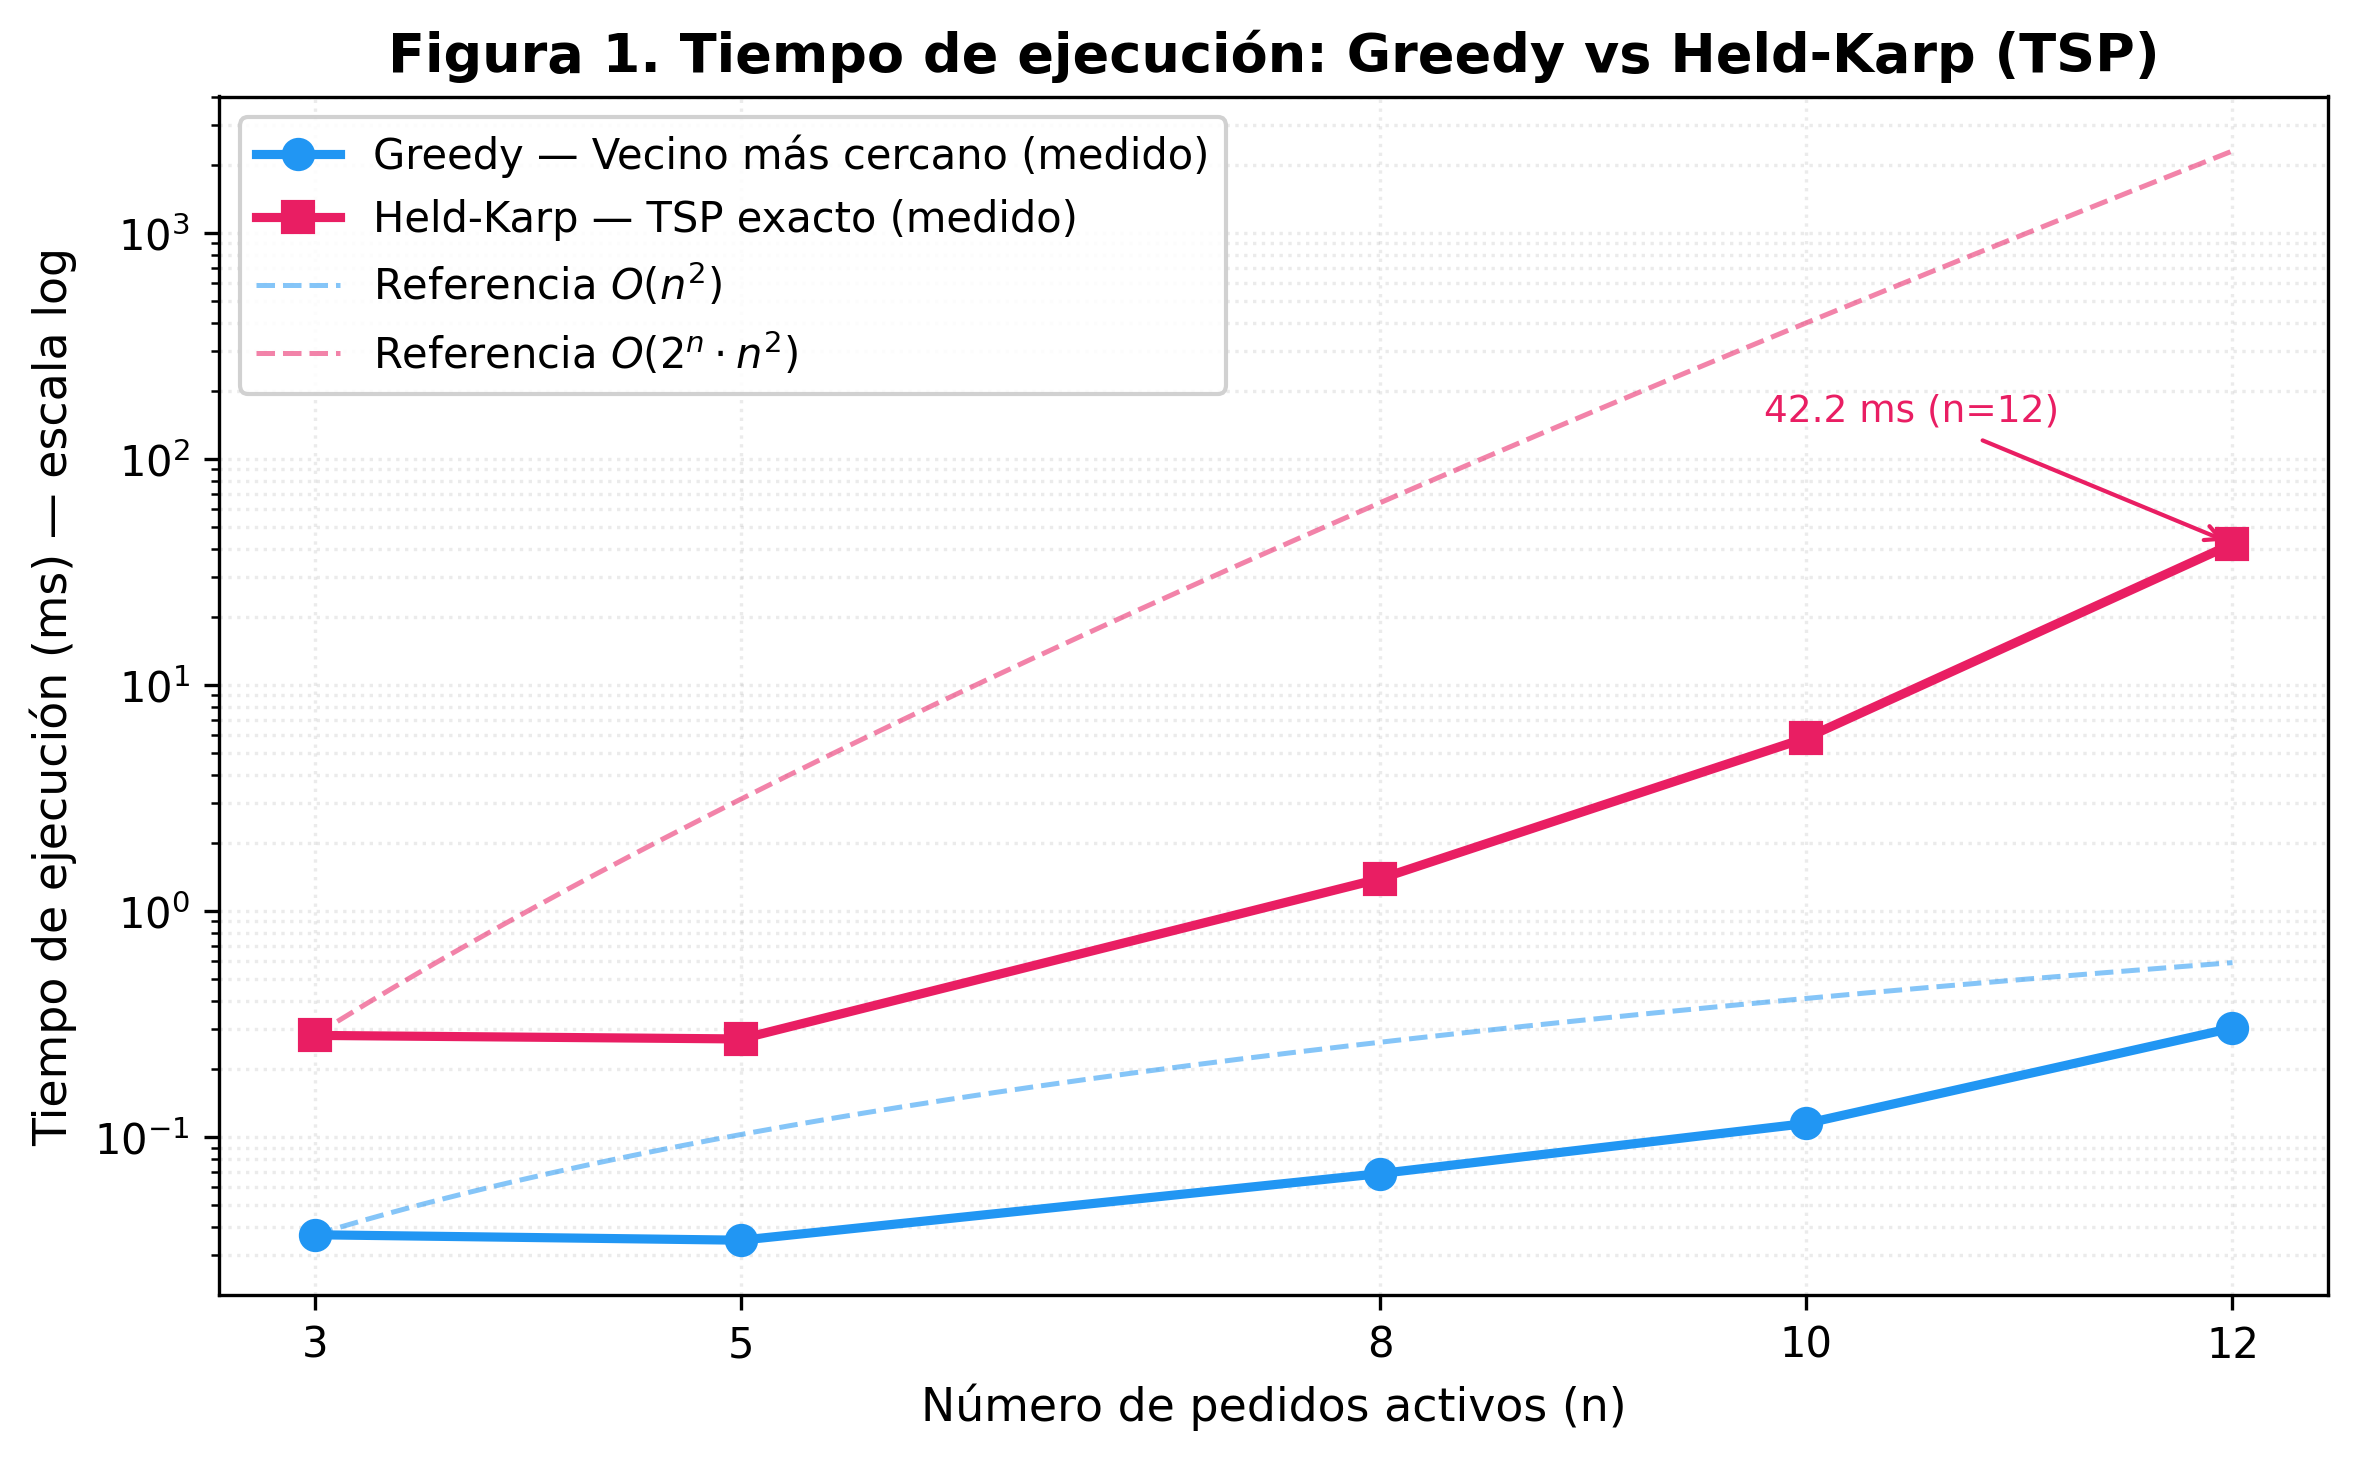
\includegraphics[width=135mm]{figuras/fig1_tiempo_vs_n.png}
\end{figure}

\subsection{Greedy frente a Held-Karp: calidad}

\begin{table}[h]
    \centering
    \caption{Distancia total del recorrido (m) y exceso del Greedy sobre el óptimo.}
    \label{tab:calidad}
    \begin{tabular}{cccc}
        \toprule
        $n$ & \textbf{Held-Karp (m)} & \textbf{Greedy (m)} & \textbf{Exceso (\%)} \\
        \midrule
        3  & 1{,}866.35  & 1{,}866.35  & 0.00  \\
        5  & 3{,}685.04  & 3{,}685.04  & 0.00  \\
        8  & 7{,}608.16  & 9{,}474.50  & 24.53 \\
        10 & 8{,}790.04  & 10{,}656.39 & 21.23 \\
        12 & 11{,}785.27 & 13{,}651.62 & 15.84 \\
        \bottomrule
    \end{tabular}
\end{table}

\begin{figure}[h]
    \centering
    \caption[Calidad de ruta: Greedy vs Held-Karp]
    {Izquierda: distancia total del recorrido (km). Derecha: exceso porcentual del Greedy sobre el óptimo.}
    \label{fig:calidad_ruta}
    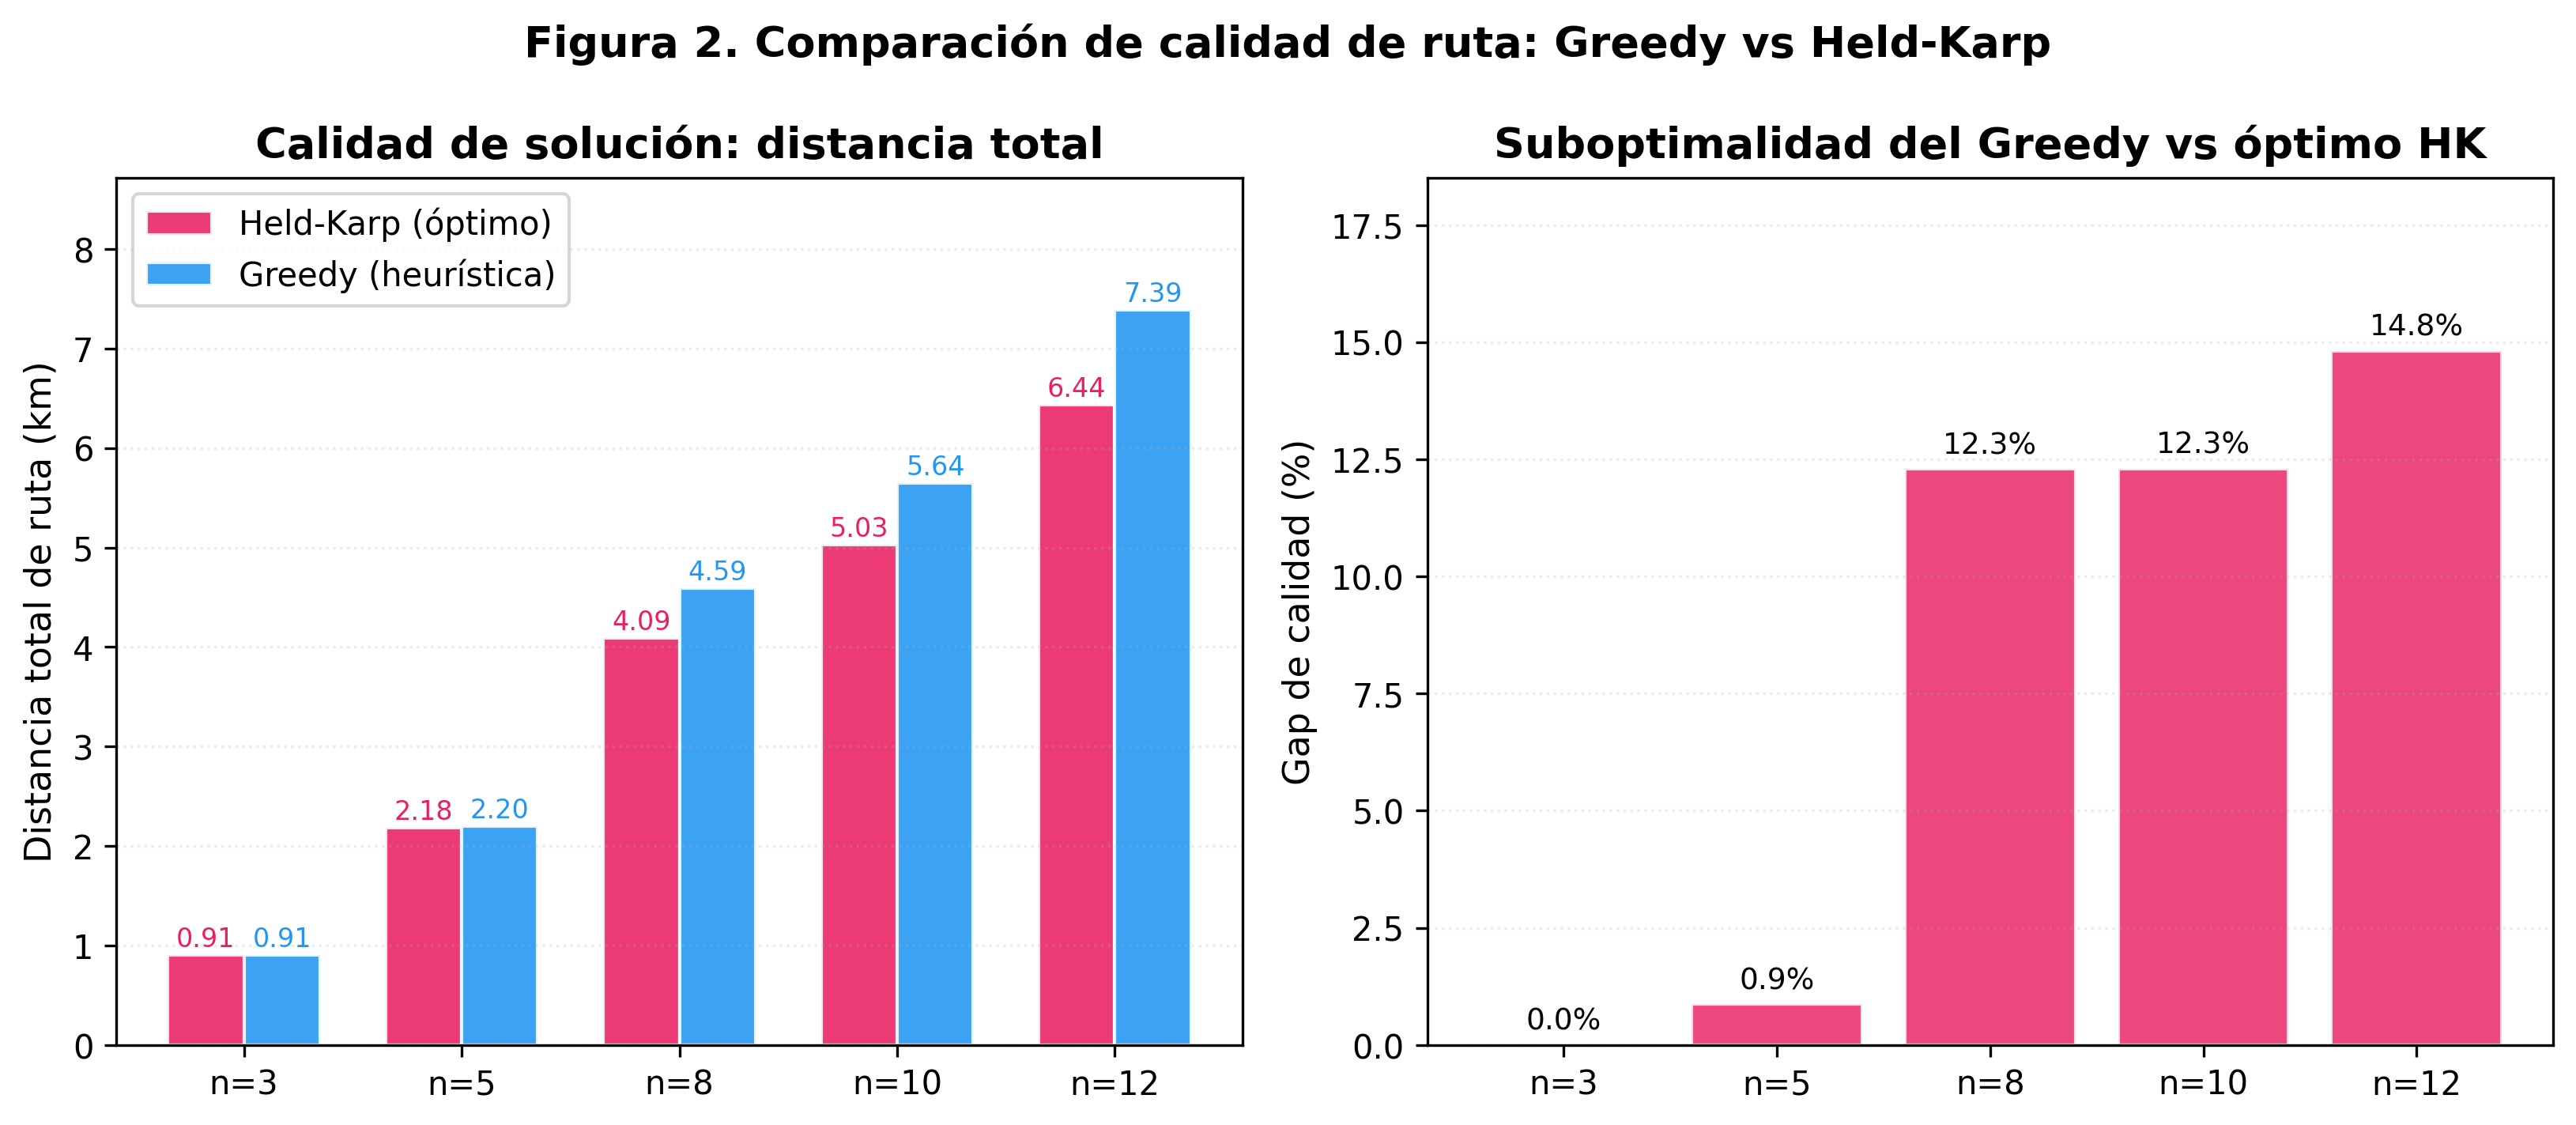
\includegraphics[width=145mm]{figuras/fig2_calidad_ruta.png}
\end{figure}

\subsection{Backtracking: todas las rutas y efecto de la poda}

En el caso del enunciado, de San Blas (N02) a Wanchaq (N11) con todas las calles abiertas, la búsqueda exhaustiva encontró \textbf{27 rutas simples}, de 1,778.62 m a 35,284.11 m. La más corta es N02$\to$N08$\to$N10$\to$N11 (1,778.62 m); la segunda, N02$\to$N09$\to$N11, mide solo 12.55 m más. Al cerrar por mantenimiento la calle San Blas--Limacpampa (N02--N08), quedan 25 rutas y el algoritmo elige N02$\to$N09$\to$N11 (1,791.17 m), sin pasar nunca por la calle cerrada.

\begin{table}[h]
    \centering
    \caption{Backtracking sin poda (exhaustivo) y con poda en cuatro pares origen--destino.}
    \label{tab:backtracking}
    \small
    \begin{tabular}{lccccccc}
        \toprule
        & \multicolumn{3}{c}{\textbf{Sin poda}} & \multicolumn{3}{c}{\textbf{Con poda}} & \\
        \cmidrule(lr){2-4}\cmidrule(lr){5-7}
        \textbf{Par} & \textbf{Rutas} & \textbf{Estados} & \textbf{ms} & \textbf{Rutas} & \textbf{Estados} & \textbf{ms} & \textbf{Óptima (m)} \\
        \midrule
        N01$\to$N04 & 1   & 776   & 0.71 & 1 & 448 & 0.41 & 790.80 \\
        N02$\to$N11 & 27  & 146   & 0.19 & 1 & 20  & 0.02 & 1{,}778.62 \\
        N01$\to$N15 & 152 & 775   & 0.92 & 2 & 142 & 0.18 & 4{,}524.34 \\
        N05$\to$N19 & 500$^{*}$ & 3{,}129 & 4.09 & 7 & 955 & 0.73 & 9{,}034.33 \\
        \bottomrule
        \multicolumn{8}{l}{\footnotesize $^{*}$ Alcanzó el tope de seguridad de 500 rutas; con poda se obtuvo la misma óptima.}
    \end{tabular}
\end{table}

La Tabla \ref{tab:backtracking} y la Figura \ref{fig:backtracking} comparan ambos modos. En los cuatro pares la ruta óptima con poda coincide con la del modo exhaustivo, como garantiza el argumento del Capítulo 4, y los estados visitados se reducen entre 42\% y 86\%. Con poda, la columna \emph{Rutas} cuenta solo las rutas que fueron mejorando la mejor distancia conocida: por eso, si se necesita la lista completa de alternativas (por ejemplo, para ofrecer una ruta de reserva), la poda debe desactivarse. El par N01$\to$N04 muestra que el número de estados no depende solo del número de rutas: hay una única ruta simple, pero la red dirigida obliga a explorar 776 estados en callejones sin salida.

\begin{figure}[h]
    \centering
    \caption[Backtracking con y sin poda]
    {Estados visitados (izquierda) y rutas registradas (derecha) por el Backtracking sin poda y con poda.}
    \label{fig:backtracking}
    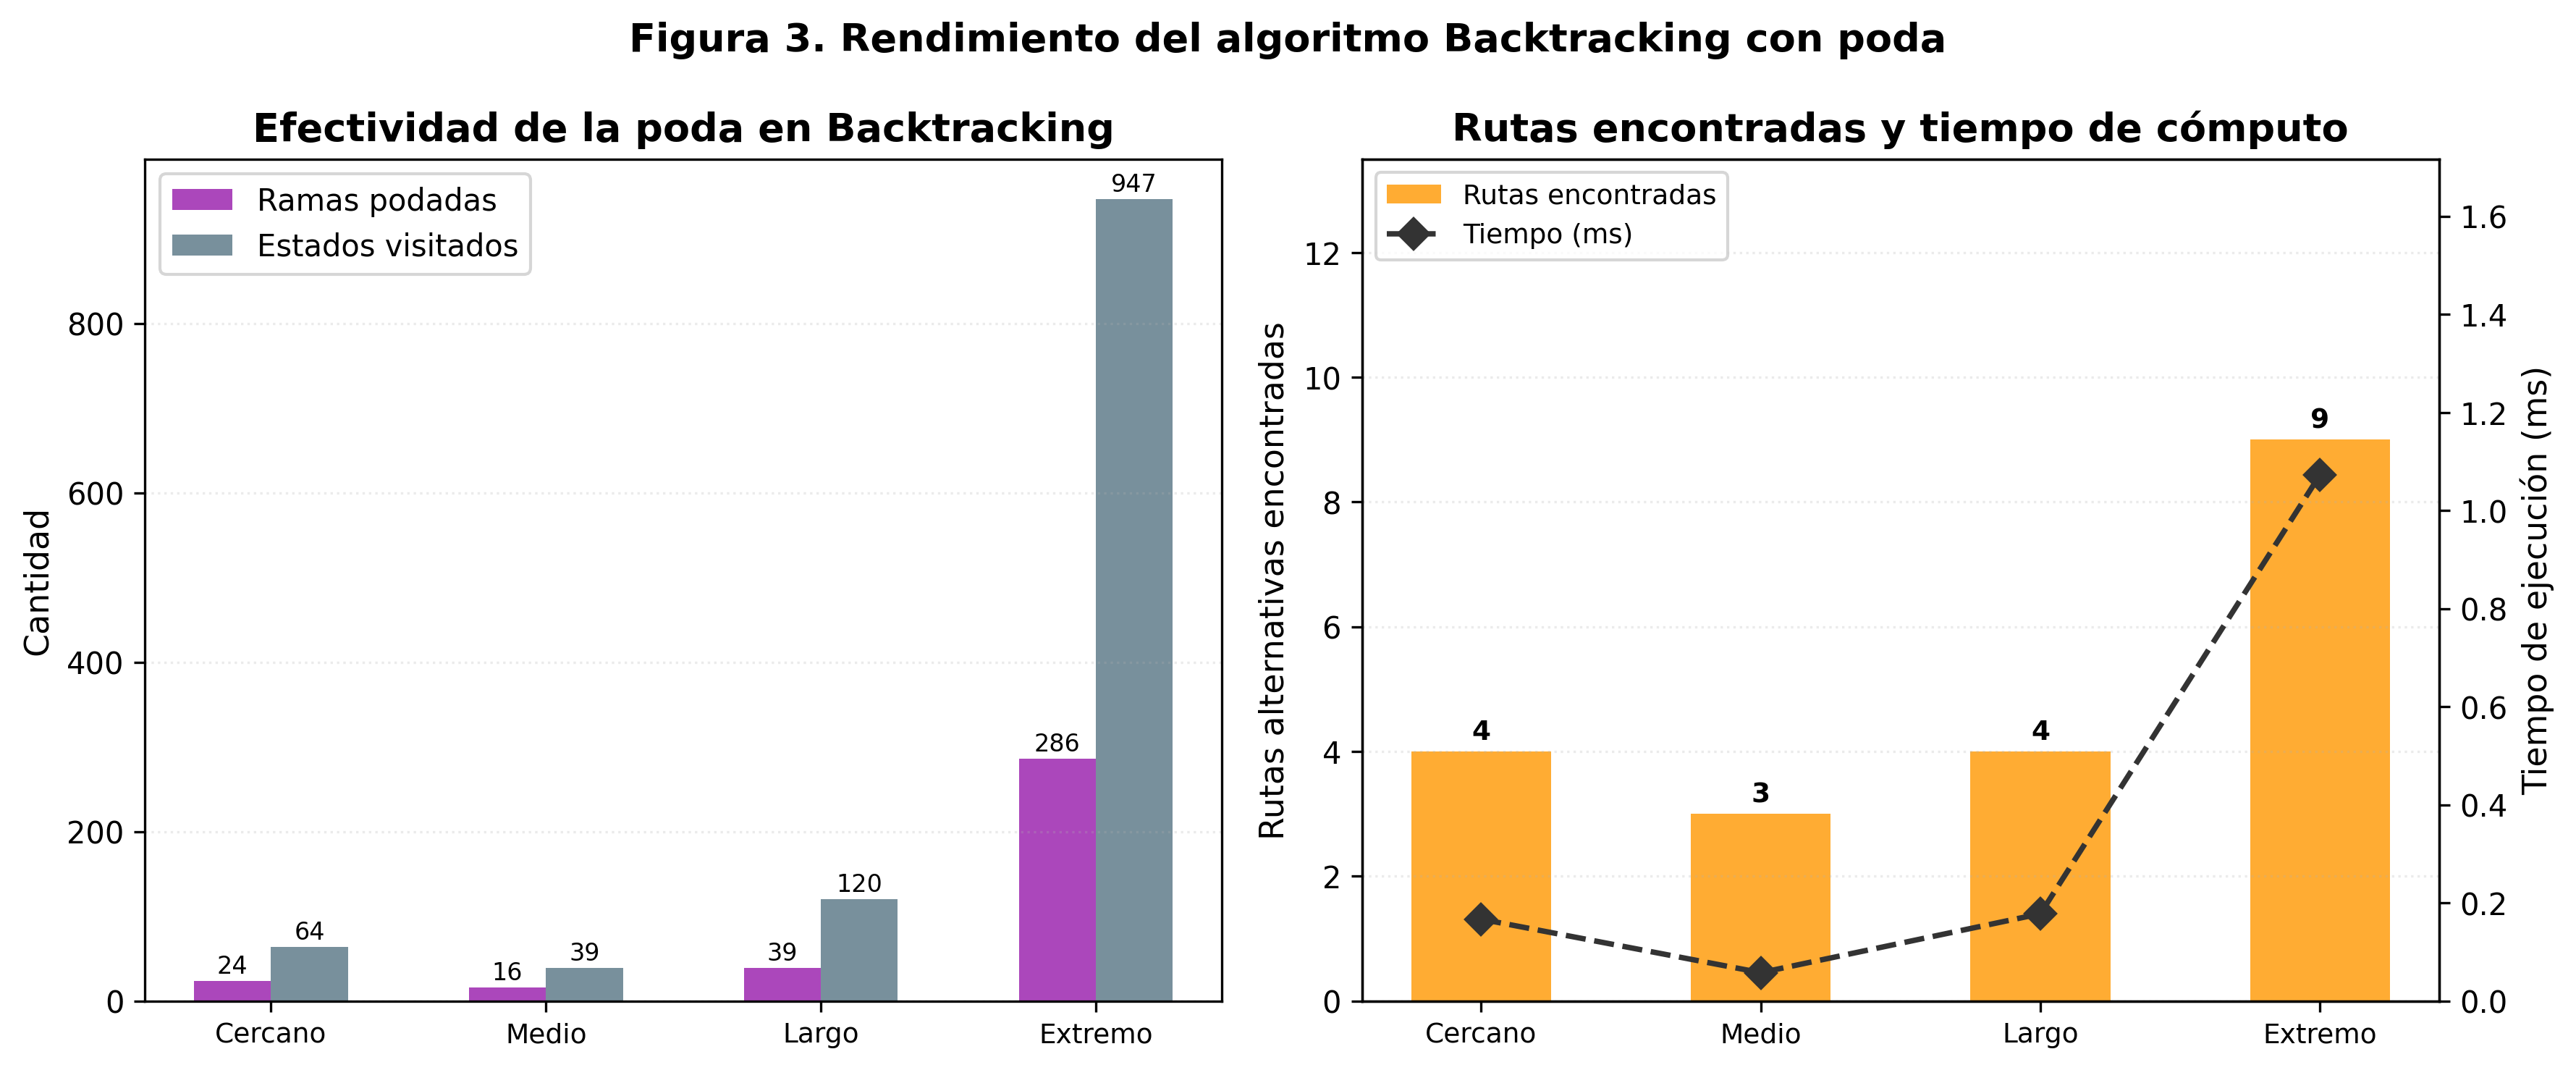
\includegraphics[width=145mm]{figuras/fig3_backtracking.png}
\end{figure}

\subsection{Mochila 0/1: Programación Dinámica frente a Greedy}

Con capacidad de 25 kg, la Mochila por PD obtuvo un valor mayor o igual al de la heurística voraz por valor/kg en todos los casos (Tabla \ref{tab:mochila}): igual con $N=5$, 10, 25 y 30, y superior con $N=15$ (S/.~1,640 frente a S/.~1,625) y $N=20$ (S/.~1,700 frente a S/.~1,695). La tabla de PD llegó a 7,781 celdas y su cálculo nunca superó 0.7 ms.

\begin{table}[h]
    \centering
    \caption{Valor cargado (S/.) con capacidad de 25 kg.}
    \label{tab:mochila}
    \begin{tabular}{cccccc}
        \toprule
        $N$ & \textbf{PD} & \textbf{Voraz} & \textbf{Celdas de la tabla} & \textbf{PD (ms)} & \textbf{Voraz (ms)} \\
        \midrule
        5  & 685   & 685   & 1{,}506 & 0.131 & 0.017 \\
        10 & 1{,}215 & 1{,}215 & 2{,}761 & 0.233 & 0.018 \\
        15 & 1{,}640 & 1{,}625 & 4{,}016 & 0.306 & 0.026 \\
        20 & 1{,}700 & 1{,}695 & 5{,}271 & 0.427 & 0.037 \\
        25 & 1{,}930 & 1{,}930 & 6{,}526 & 0.492 & 0.043 \\
        30 & 2{,}365 & 2{,}365 & 7{,}781 & 0.602 & 0.058 \\
        \bottomrule
    \end{tabular}
\end{table}

Durante la revisión se detectó y corrigió un error en la discretización de pesos: la versión inicial redondeaba cada peso al kilogramo más cercano (2.2 kg contaba como 2 kg y 4.5 kg como 4 kg), y con los 15 primeros pedidos llegó a elegir 5.2 kg para una capacidad de 5 kg y 15.2 kg para una de 15 kg. La versión final trabaja con precisión de 0.1 kg, redondea los pesos hacia arriba y la capacidad hacia abajo, y una prueba automática verifica que la carga nunca exceda la capacidad.

\subsection{Divide y Vencerás}

\textbf{Una zona por repartidor.} Con los 30 pedidos y los 3 repartidores, la partición produjo tres zonas de 10 pedidos y cada repartidor calculó con Held-Karp la ruta óptima de su zona (Tabla \ref{tab:zonas}). Entre los tres recorren 30.22 km, frente a 43.35 km de un único repartidor que atiende todo con el Greedy; además trabajan en paralelo, por lo que el reparto termina cuando acaba la ruta más larga (12.46 km).

\begin{table}[h]
    \centering
    \caption{Divide y Vencerás: una zona por repartidor (30 pedidos).}
    \label{tab:zonas}
    \begin{tabular}{llcc}
        \toprule
        \textbf{Zona} & \textbf{Repartidor} & \textbf{Pedidos} & \textbf{Ruta óptima (m)} \\
        \midrule
        1 & REP-03 (furgoneta, Marcavalle)       & 10 & 12{,}457.73 \\
        2 & REP-01 (bicicleta, Plaza de Armas)   & 10 & 11{,}974.11 \\
        3 & REP-02 (motocicleta, Av. El Sol)     & 10 & 5{,}788.10 \\
        \midrule
        \multicolumn{3}{l}{Total del equipo} & 30{,}219.94 \\
        \multicolumn{3}{l}{Un solo repartidor (Greedy, desde la Plaza de Armas)} & 43{,}352.76 \\
        \bottomrule
    \end{tabular}
\end{table}

\textbf{Un repartidor y zonas de $K$ pedidos.} Con pedidos sintéticos (Figura \ref{fig:mochila_dyv}, derecha, y Anexo E), el tiempo de Divide y Vencerás con $K=5$ pasó de 0.22 ms ($n=30$) a 11.6 ms ($n=480$), similar al del Greedy global. Sin embargo, su ruta fue más larga para $n\ge60$: como los pedidos se concentran en solo 20 lugares, el corte por coordenadas separa en zonas distintas pedidos de un mismo lugar y obliga a volver a él, mientras que el Greedy los atiende todos de una vez. Para un único repartidor, la segmentación sirve para organizar el trabajo, no para acortar la ruta; su ventaja aparece al repartir zonas entre varios repartidores.

\begin{figure}[h]
    \centering
    \caption[Mochila y Divide y Vencerás]
    {Izquierda: valor cargado por la Mochila con PD y por la heurística voraz. Derecha: rutas de las tres zonas frente a un único repartidor voraz.}
    \label{fig:mochila_dyv}
    \includegraphics[width=145mm]{figuras/fig4_mochila_dyv.png}
\end{figure}

\subsection{Verificación de correctitud y estabilidad}

Las 39 pruebas unitarias de \texttt{tests/} se aprobaron sin fallos (Anexo C). La prueba automática de la interfaz ejecutó todas las funcionalidades de las siete pestañas, incluido el \textit{benchmark} en vivo, sin errores ni bloqueos; las capturas del Anexo D proceden de esa ejecución.

\section{Discusión: ¿cuándo usar cada enfoque?}

\textbf{Greedy frente a Programación Dinámica en rutas.} Held-Karp garantiza el recorrido óptimo, pero por su costo $O(n^2 2^n)$ su tiempo se multiplicó por 376 entre $n=5$ y $n=12$, hasta 22 ms; el Greedy respondió siempre en menos de 0.05 ms, pero produjo recorridos hasta 24.5\% más largos. Por tanto, conviene PD cuando el número de paradas es pequeño ($n \le 12$--14) y el ahorro de distancia importa, por ejemplo en la ruta del día de cada repartidor o dentro de cada zona de Divide y Vencerás. Conviene el Greedy cuando hay muchas paradas, cuando la respuesta debe ser inmediata (pedidos de emergencia) o cuando la ruta se recalcula continuamente.

\textbf{Greedy frente a Programación Dinámica en la carga.} En la mochila la PD resulta casi siempre preferible: su costo $O(N\cdot W)$ es pseudo-polinomial y, con capacidades reales de vehículos, la tabla tiene unos pocos miles de celdas y se calcula en menos de 1 ms. La heurística voraz solo tendría sentido con capacidades enormes o precisión muy fina, donde $W$ haría crecer demasiado la tabla.

\textbf{Backtracking.} Es el único enfoque que enumera \emph{todas} las alternativas y admite cualquier restricción (calles cerradas, sentidos, tramos obligatorios). Su costo es exponencial: en la red de 20 lugares se mantiene por debajo de 5 ms, pero el par N05$\to$N19 ya supera las 500 rutas simples. Conviene cuando el grafo es pequeño o la zona de búsqueda está acotada, cuando se necesitan rutas de reserva, o con la poda activada cuando solo interesa la ruta óptima bajo restricciones.

\textbf{Divide y Vencerás.} Su aporte es dividir el trabajo: al asignar una zona a cada repartidor, cada subproblema queda lo bastante pequeño para resolverse de forma exacta, y el equipo recorre 30\% menos distancia que un único repartidor. Para un solo vehículo no mejora la calidad de la ruta.

En conjunto, los paradigmas no compiten sino que se complementan. El sistema combina Divide y Vencerás para repartir zonas, PD para cargar cada vehículo y ordenar cada zona, Greedy para las decisiones urgentes y Backtracking cuando las restricciones de la red vial obligan a buscar alternativas.

\chapter{Conclusiones y Recomendaciones}

\section{Conclusiones}

\begin{itemize}
    \item \textbf{Sobre la implementación algorítmica:} se implementaron desde cero, sin librerías de optimización ni de grafos, los cuatro paradigmas exigidos y aplicados a los casos de uso del enunciado: Greedy para la ruta voraz y la asignación de emergencias; Divide y Vencerás para segmentar la ciudad en una zona por repartidor; Programación Dinámica para cargar el vehículo (Mochila 0/1) y obtener el recorrido exacto (Held-Karp); y Backtracking para encontrar todas las rutas de San Blas a Wanchaq evitando calles cerradas. Su correctitud está respaldada por 39 pruebas unitarias con resultados esperados calculados de forma independiente.

    \item \textbf{Sobre la complejidad:} las mediciones concuerdan con el análisis Big-O. El tiempo de Held-Karp, $O(n^2 2^n)$, se multiplicó por 376 entre 5 y 12 puntos, mientras que el Greedy, $O(n^2)$, se mantuvo por debajo de 0.05 ms. El análisis también corrigió dos estimaciones iniciales: la partición de Divide y Vencerás cuesta $\Theta(n\log^2 n)$, no $\Theta(n\log n)$, porque en cada nivel se ordena; y su variante con un solo repartidor cuesta $O(n^2/K)$ por la elección voraz entre zonas.

    \item \textbf{Sobre la calidad de las soluciones:} el Greedy produjo recorridos hasta 24.5\% más largos que el óptimo, y la mochila voraz cargó hasta S/.~15 menos que la PD. La poda del Backtracking redujo los estados visitados entre 42\% y 86\% sin perder la ruta óptima. Dividir la ciudad en una zona por repartidor redujo la distancia total de 43.4 a 30.2 km.

    \item \textbf{Sobre el sistema:} la aplicación ejecuta todas sus funcionalidades sin bloquearse, gracias a los cálculos en segundo plano y al manejo centralizado de errores; funciona sin conexión a Internet con un mapa vectorial propio; y permite cerrar calles y observar su efecto en todos los algoritmos. Una prueba automática de la interfaz recorre todas las pestañas y respalda esta afirmación.
\end{itemize}

\section{Recomendaciones}

\begin{itemize}
    \item Para escalar a más de 14 paradas, sustituir Held-Karp por heurísticas de mejora como 2-opt aplicadas sobre la ruta del Greedy, que reducen el exceso de distancia en tiempo polinomial.
    \item Incorporar el volumen como segunda restricción de la mochila, con una tabla $dp[i][w][v]$ de costo $O(N\cdot W\cdot V)$; actualmente el volumen solo se verifica después de optimizar por peso.
    \item Calcular la mediana por selección lineal (Quickselect) en lugar de ordenar en cada nivel, para que la partición espacial baje de $\Theta(n\log^2 n)$ a $\Theta(n\log n)$.
    \item Revisar en campo los ocho lugares cuya ubicación se desplazó más de 60 m al ajustarse a la red vial (Anexo B) y reconstruir el caché vial con las coordenadas corregidas.
    \item Añadir persistencia de pedidos (por ejemplo, SQLite) y tiempos de viaje por tipo de vehículo, para que la herramienta pueda usarse en la operación diaria de una empresa de reparto.
\end{itemize}


%%%%%%%%%%%%%%%%%%%%%%%%%%%%%%%%%%%%%%%%%%%%%%%%%%%%%%%%%%%%%%%%%%%%%%
% Referencias bibliográficas
\bibliographystyle{apalike}
\bibliography{contenido/bibliog}
\addcontentsline{toc}{chapter}{Referencias}

% Apéndice y anexos
\chapter*{Apéndice y Anexos}
\addcontentsline{toc}{chapter}{Apéndice y Anexos}

\section*{Anexo A: Estructura del Repositorio}

\begin{verbatim}
proyecto-progra-iii/
|-- main.py                  # Punto de entrada de la aplicacion
|-- config.py                # Parametros globales (mapa, colores, limites)
|-- requirements.txt         # Dependencias de la aplicacion
|-- requirements-dev.txt     # Dependencias para reconstruir la red vial
|-- core/                    # Algoritmos y modelo (sin interfaz grafica)
|   |-- modelos.py           # Nodo, Arista, Pedido, Repartidor, Ruta, Grafo
|   |-- grafo.py             # Dijkstra, matriz de distancias, caminos
|   |-- geo.py               # Haversine y asignacion al lugar mas cercano
|   |-- estructuras.py       # Merge/Quick Sort, busqueda binaria, indices
|   |-- greedy.py            # Vecino mas cercano, emergencia, mochila voraz
|   |-- divide_venceras.py   # Particion en zonas de K y en R zonas
|   |-- prog_dinamica.py     # Mochila 0/1 y Held-Karp
|   |-- backtracking.py      # Rutas simples con poda opcional
|   +-- gestor_datos.py      # Carga de JSON
|-- gui/
|   |-- app.py               # Ventana principal, errores y barra de estado
|   |-- tab_mapa.py          # Red vial y cierre de calles
|   |-- tab_pedidos.py       # Ordenacion, busqueda y alta de pedidos
|   |-- tab_greedy.py        # Pestana Greedy
|   |-- tab_dyv.py           # Pestana Divide y Venceras
|   |-- tab_pd.py            # Pestana Mochila y Held-Karp
|   |-- tab_backtracking.py  # Pestana Backtracking
|   |-- tab_comparacion.py   # Graficos y tabla Big-O
|   |-- componente_mapa.py   # Mapa (tkintermapview o Canvas sin conexion)
|   |-- canvas_fallback.py   # Mapa vectorial sin conexion
|   |-- hilos.py             # Calculos en segundo plano
|   +-- panel_desplazable.py # Paneles laterales con desplazamiento
|-- data/                    # red_vial_cache.json, pedidos.json, repartidores.json
|-- benchmarks/              # benchmark.py y resultados_benchmark.json
|-- tests/                   # 39 pruebas pytest
|-- tools/                   # Construccion de la red vial y prueba de la GUI
+-- informe/                 # Este informe (LaTeX) y generar_figuras.py
\end{verbatim}

\section*{Anexo B: Lugares de Interés de la Red Vial}

Coordenadas ajustadas a la intersección vial más cercana (OpenStreetMap, 19/10/2026). La última columna indica cuánto se desplazó cada lugar respecto de su coordenada original; $^{*}$ marca desplazamientos mayores a 60 m, pendientes de revisión.

\begin{table}[h]
    \centering
    \caption{Lugares de interés del grafo vial de Cusco.}
    \label{tab:nodos}
    \footnotesize
    \begin{tabular}{lllccr}
        \toprule
        \textbf{ID} & \textbf{Nombre} & \textbf{Sector} & \textbf{Lat} & \textbf{Lon} & \textbf{Ajuste (m)} \\
        \midrule
        N01 & Plaza de Armas & Centro Histórico & $-13.51653$ & $-71.97961$ & 89.8$^{*}$ \\
        N02 & San Blas & Centro Histórico & $-13.51503$ & $-71.97478$ & 30.5 \\
        N03 & Coricancha & Centro Histórico & $-13.51991$ & $-71.97561$ & 64.6$^{*}$ \\
        N04 & Mercado San Pedro & Centro Histórico & $-13.52041$ & $-71.98316$ & 117.7$^{*}$ \\
        N05 & Plaza Santiago & Santiago & $-13.52327$ & $-71.98586$ & 34.0 \\
        N06 & Santa Ana & Santiago & $-13.51760$ & $-71.98823$ & 27.5 \\
        N07 & Sacsayhuamán Acceso & Centro Histórico & $-13.50771$ & $-71.98014$ & 267.9$^{*}$ \\
        N08 & Limacpampa & Centro Histórico & $-13.51943$ & $-71.97362$ & 123.0$^{*}$ \\
        N09 & Lucrepata & Wanchaq & $-13.51789$ & $-71.96903$ & 13.0 \\
        N10 & Av. El Sol (Cruce Pardo) & Wanchaq & $-13.52348$ & $-71.97196$ & 5.3 \\
        N11 & Wanchaq (Estación) & Wanchaq & $-13.52475$ & $-71.96853$ & 7.1 \\
        N12 & Plaza Túpac Amaru & Wanchaq & $-13.52264$ & $-71.96374$ & 30.0 \\
        N13 & Ttio La Florida & Wanchaq & $-13.53055$ & $-71.95937$ & 14.9 \\
        N14 & Hospital Regional & Wanchaq & $-13.52511$ & $-71.95612$ & 45.4 \\
        N15 & Av. Cultura (UNSAAC) & Wanchaq & $-13.52698$ & $-71.95139$ & 11.8 \\
        N16 & Cuatro Torpes & San Sebastián & $-13.53142$ & $-71.94814$ & 66.6$^{*}$ \\
        N17 & Magisterio & San Sebastián & $-13.52840$ & $-71.94183$ & 21.5 \\
        N18 & Marcavalle & San Sebastián & $-13.52984$ & $-71.93343$ & 46.5 \\
        N19 & Plaza San Sebastián & San Sebastián & $-13.53256$ & $-71.92627$ & 76.5$^{*}$ \\
        N20 & San Jerónimo Entrada & San Sebastián & $-13.54129$ & $-71.90449$ & 64.1$^{*}$ \\
        \bottomrule
    \end{tabular}
\end{table}

\clearpage
\section*{Anexo C: Resultados de Pruebas Unitarias}

{\scriptsize
\begin{verbatim}
$ pytest -v
tests/test_backtracking.py::test_backtracking_dos_rutas_y_optima PASSED
tests/test_backtracking.py::test_backtracking_con_calle_bloqueada PASSED
tests/test_backtracking.py::test_backtracking_sin_conexion PASSED
tests/test_backtracking.py::test_backtracking_poda_por_costo PASSED
tests/test_backtracking.py::test_sin_poda_enumera_todas_las_rutas_san_blas_wanchaq PASSED
tests/test_backtracking.py::test_sin_poda_respeta_calles_cerradas PASSED
tests/test_dyv.py::test_particion_tamanios_menores_o_iguales_a_k PASSED
tests/test_dyv.py::test_resolver_rutas_dyv_ensamble PASSED
tests/test_dyv.py::test_particion_en_r_zonas_exactas PASSED
tests/test_dyv.py::test_un_repartidor_por_zona PASSED
tests/test_dyv.py::test_held_karp_por_zona_no_peor_que_greedy PASSED
tests/test_estructuras.py::test_merge_sort_numeros PASSED
tests/test_estructuras.py::test_merge_sort_reverse PASSED
tests/test_estructuras.py::test_merge_sort_pedidos_por_valor PASSED
tests/test_estructuras.py::test_quick_sort_numeros PASSED
tests/test_estructuras.py::test_quick_sort_con_duplicados PASSED
tests/test_estructuras.py::test_quick_sort_pedidos_por_prioridad PASSED
tests/test_estructuras.py::test_busqueda_binaria_exito_y_fallo PASSED
tests/test_estructuras.py::test_busqueda_binaria_en_pedidos PASSED
tests/test_estructuras.py::test_indices_hash_e_invertido PASSED
tests/test_grafo.py::test_dijkstra_reconstruye_optimo_en_grafo_pequeno PASSED
tests/test_grafo.py::test_geometria_de_ruta_concatena_curvas_en_sentido_correcto PASSED
tests/test_grafo.py::test_asignacion_de_coordenada_elige_nodo_mas_cercano_por_haversine PASSED
tests/test_grafo.py::test_cierre_actualiza_matriz_y_puede_hacer_inalcanzable PASSED
tests/test_grafo.py::test_cierre_bidireccional_cierra_arcos_en_ambos_sentidos PASSED
tests/test_grafo.py::test_cache_es_fuertemente_conexo_y_cumple_desigualdad_triangular PASSED
tests/test_grafo.py::test_cache_aristas_tienen_peso_mayor_que_recta_y_geometria_con_extremos PASSED
tests/test_greedy.py::test_vecino_cercano_orden_esperado PASSED
tests/test_greedy.py::test_vecino_cercano_con_retorno PASSED
tests/test_greedy.py::test_vecino_cercano_respeta_distancias_asimetricas PASSED
tests/test_greedy.py::test_asignacion_emergencia_mas_cercano PASSED
tests/test_greedy.py::test_asignacion_emergencia_filtro_por_capacidad PASSED
tests/test_pd.py::test_mochila_caso_clasico_libro PASSED
tests/test_pd.py::test_mochila_capacidad_cero_o_vacio PASSED
tests/test_pd.py::test_held_karp_tsp_triangulo_retorno PASSED
tests/test_pd.py::test_held_karp_tsp_4_puntos PASSED
tests/test_pd.py::test_mochila_pesos_decimales_no_exceden_capacidad PASSED
tests/test_pd.py::test_mochila_datos_reales_respetan_capacidad PASSED
tests/test_pd.py::test_mochila_coincide_con_fuerza_bruta PASSED

============================== 39 passed ==============================
\end{verbatim}
}

\clearpage
\section*{Anexo D: Capturas de la Interfaz Gráfica}

Capturas tomadas por \texttt{tools/prueba\_gui.py} en modo sin conexión (mapa vectorial en \texttt{Canvas}). Con conexión a Internet, el mapa muestra además los tiles de OpenStreetMap.

\begin{figure}[!htbp]
    \centering
    \caption[Pestaña Red Vial]{Pestaña Red Vial: los 20 lugares y las conexiones por calles, con controles para cerrar calles y tabla de desvío (línea recta frente a calles).}
    \includegraphics[width=150mm]{figuras/gui/captura_01_mapa_inicial.png}
\end{figure}

\begin{figure}[!htbp]
    \centering
    \caption[Pestaña Pedidos]{Pestaña Pedidos: pedidos ordenados por prioridad con Merge Sort manual; colores por urgencia y búsqueda por ID o sector.}
    \includegraphics[width=150mm]{figuras/gui/captura_02_tabla_pedidos.png}
\end{figure}
\clearpage

\begin{figure}[!htbp]
    \centering
    \caption[Pestaña Greedy]{Pestaña Greedy: ruta del vecino más cercano para 8 pedidos, con las entregas numeradas en el orden elegido.}
    \includegraphics[width=150mm]{figuras/gui/captura_03_ruta_greedy.png}
\end{figure}

\begin{figure}[!htbp]
    \centering
    \caption[Pestaña Divide y Vencerás]{Pestaña Divide y Vencerás: tres zonas, una por repartidor, cada una con su ruta óptima.}
    \includegraphics[width=150mm]{figuras/gui/captura_04_dyv_repartidores.png}
\end{figure}
\clearpage

\begin{figure}[!htbp]
    \centering
    \caption[Pestaña Programación Dinámica]{Pestaña Programación Dinámica: Held-Karp (púrpura) frente a Greedy (verde) sobre los mismos 8 puntos.}
    \includegraphics[width=150mm]{figuras/gui/captura_05_ruta_held_karp.png}
\end{figure}

\begin{figure}[!htbp]
    \centering
    \caption[Pestaña Backtracking]{Pestaña Backtracking: San Blas a Wanchaq con la calle N02--N08 cerrada (rojo) y la nueva ruta más corta (azul).}
    \includegraphics[width=150mm]{figuras/gui/captura_06_backtracking_bloqueo.png}
\end{figure}
\clearpage

\begin{figure}[!htbp]
    \centering
    \caption[Pestaña Programación Dinámica]{Pestaña Programación Dinámica: Mochila 0/1 con la capacidad de la bicicleta, tabla DP con los pedidos elegidos resaltados y comparación con el voraz.}
    \includegraphics[width=150mm]{figuras/gui/captura_07_knapsack_seleccion.png}
\end{figure}

\begin{figure}[!htbp]
    \centering
    \caption[Pestaña Comparación]{Pestaña Comparación: gráficos de los benchmarks, tabla Big-O y conclusiones calculadas a partir de los datos.}
    \includegraphics[width=150mm]{figuras/gui/captura_08_comparacion.png}
\end{figure}
\clearpage

\section*{Anexo E: Divide y Vencerás con un Repartidor (Pedidos Sintéticos)}

Pedidos sintéticos (semilla 2026) ubicados en los 20 lugares con una pequeña variación de coordenadas; partida desde la Plaza de Armas y $K=5$.

\begin{table}[h]
    \centering
    \caption{Divide y Vencerás ($K=5$) frente a Greedy global con un repartidor.}
    \label{tab:dyv_sintetico}
    \begin{tabular}{ccccc}
        \toprule
        $n$ & \textbf{D\&C (ms)} & \textbf{Greedy (ms)} & \textbf{Distancia D\&C (m)} & \textbf{Distancia Greedy (m)} \\
        \midrule
        30 & 0.215 & 0.054 & 40{,}912 & 40{,}715 \\
        60 & 0.579 & 0.160 & 53{,}636 & 43{,}353 \\
        120 & 1.240 & 0.599 & 57{,}637 & 43{,}353 \\
        240 & 3.527 & 2.919 & 75{,}611 & 43{,}353 \\
        480 & 11.581 & 10.492 & 106{,}593 & 43{,}353 \\
        \bottomrule
    \end{tabular}
\end{table}

\addcontentsline{toc}{chapter}{Apéndice y Anexos}
\end{document}
